% Ce fichier main.tex est le fichier principal \`{a} partir duquel tout est g\'{e}n\'{e}r\'{e}
% This file is the main file where the final document is generated
\documentclass{these-dbl}

% Fill the pdf metadata
\hypersetup{
%    pdfauthor   = {XYZ},
%    pdftitle    = {Th\`{e}se de doctorat de XYZ},
%    pdfsubject  = {Th\`{e}se de doctorat de XYZ},
%    pdfkeywords = {mots-cl\'{e}s},
}

\geometry{vmargin=4.0cm}
\addbibresource{./biblio/biblio.bib}

\makeglossaries
% Acronymes
\newacronym{gcd}{GCD}{Greatest Common Divisor}
\newacronym{lcm}{LCM}{Least Common Multiple}

% Définitions
\newglossaryentry{git}
{
    name={git},
    description={
    Logiciel de versionnage git, raccourcit pour désigner à la fois un répertoire git ou un projet git sur des plateformes en ligne comme github ou gitlab.
    }
    name={git},
    description={
    Logiciel de versionnage git, raccourcit pour désigner à la fois un répertoire git ou un projet git sur des plateformes en ligne comme github ou gitlab.
    }
    name={git},
    description={
    Logiciel de versionnage git, raccourcit pour désigner à la fois un répertoire git ou un projet git sur des plateformes en ligne comme github ou gitlab.
    }
    name={git},
    description={
    Logiciel de versionnage git, raccourcit pour désigner à la fois un répertoire git ou un projet git sur des plateformes en ligne comme github ou gitlab.
    }
    name={git},
    description={
    Logiciel de versionnage git, raccourcit pour désigner à la fois un répertoire git ou un projet git sur des plateformes en ligne comme github ou gitlab.
    }
    name={git},
    description={
    Logiciel de versionnage git, raccourcit pour désigner à la fois un répertoire git ou un projet git sur des plateformes en ligne comme github ou gitlab.
    }
    name={git},
    description={
    Logiciel de versionnage git, raccourcit pour désigner à la fois un répertoire git ou un projet git sur des plateformes en ligne comme github ou gitlab.
    }
    name={git},
    description={
    Logiciel de versionnage git, raccourcit pour désigner à la fois un répertoire git ou un projet git sur des plateformes en ligne comme github ou gitlab.
    }
}

\begin{document}

% La page de garde est en français
% The front cover is in French
\selectlanguage{english}

\maketitle



\selectlanguage{spanish}

\clearemptydoublepage
\chapter*{Agradecimientos}

Me gustaría dar las gracias a todos los que me han apoyado durante este programa de intercambio universitario y el periodo de prácticas.

A mi familia por enseñarme siempre a apuntar lo más alto posible. Todo lo que han hecho ha sido para ayudarme a crecer. También les agradezco su apoyo material durante este periodo; sin él, no podría haberlo conseguido.

A mis amigos, tanto los de casa como los nuevos que he ido conociendo por el camino, por animarme y aconsejarme siempre desde cualquier parte del mundo.

A mi supervisor y mis compañeros, por confiar en mí y en mi criterio para encontrar la mejor solución posible para cada tarea asignada. Todos ellos demostraron ser ejemplares a su manera.

A mis universidades de Francia y Argentina, por darme los conocimientos y las herramientas necesarias para perseguir mis sueños como joven profesional.

A mi profesor tutor de Proyecto Final de Estudios, por aconsejarme y acompañarme en este proceso.

\frontmatter
\clearemptydoublepage
\renewcommand{\contentsname}{Tabla de Contenidos}
\tableofcontents %sommaire %table of content
%\shorttableofcontents{Sommaire}{0}

\clearemptydoublepage
\listoffigures

\clearemptydoublepage
\chapter*{Resumen}
\addcontentsline{toc}{chapter}{Resumen}
\chaptermark{Resumen}

Este documento consiste en el informe de mi Proyecto Final de Estudios realizado durante mi período de prácticas en el instituto Fraunhofer IPK en Berlín, Alemania. Mi período en este instituto fue de 6 meses y aquí expondré los resultados de mi trabajo.

En el ámbito científico, trabajar con ontologías es parte del día a día y los software para hacerlo no cuentan con suficientes herramientas. En este contexto, Gaia-X busca desarrollar un estándar de información a nivel europeo para asegurarse la portabilidad y gobernanza. Para brindarles una opción extra a la hora de manipular las ontologías de su proyecto, desarrollamos una aplicación en Realidad Virtual con el objetivo de simplificar algunas tareas.
Aquí intentaré explicar lo más claramente posible cuál fue mi trabajo dentro del proyecto y el resultado de estos 6 meses.

El proyecto continúa una vez finalizadas mis prácticas, pero la simulación es estable y sigue en marcha, con mucho trabajo por hacer. En este informe mostraré una parte del proceso de desarrollo de las funciones que me asignaron.
El trabajo futuro incluye planificar y desarrollar más funciones, así como probar y pulir la experiencia del usuario.


\clearemptydoublepage
\chapter*{Introducción}
\addcontentsline{toc}{chapter}{Introducción}
\chaptermark{Introducción}


La velocidad a la que evoluciona la tecnología es cada vez mayor, por lo que necesitamos seguir desarrollando software
y crear aplicaciones para aprovechar al máximo las herramientas de que disponemos. Una de estas tecnologías es la
Realidad Extendida (XR - \textit{Extended Reality}) con todos sus niveles de interacción y, para cada tarea, necesitamos encontrar la respuesta mas adecuada a las necesidades.

En este informe voy a mostrar los resultados del proyecto realizado durante mi periodo de práctica profesional dentro del instituto Fraunhofer IPK en Berlín, Alemania.
Para ello, voy a exponer los grandes bloques conceptuales que componen este proyecto, el estado del arte actual, el trabajo realizado, ejemplos de código, esquemas de datos y conclusiones personales.

\begin{figure}[ht]
    \begin{center}
       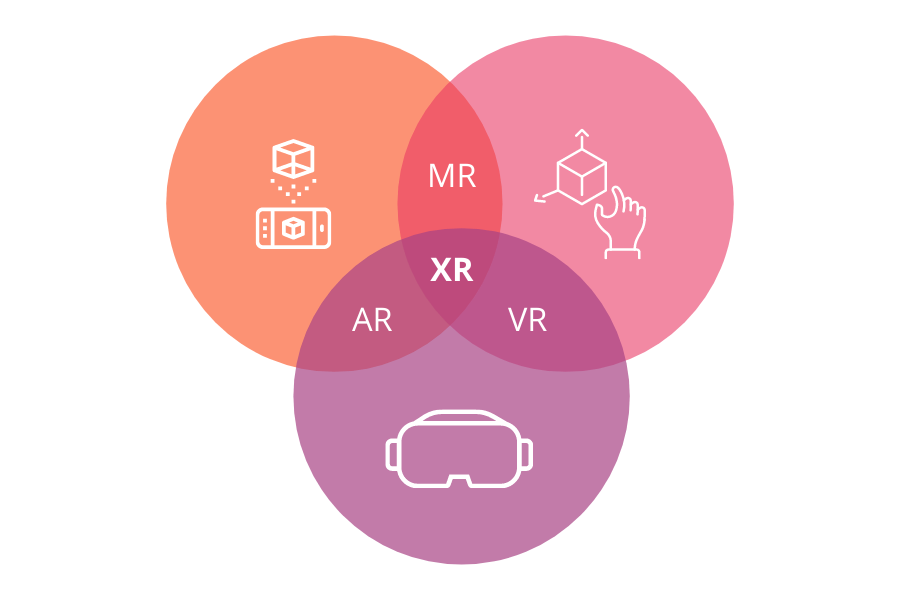
\includegraphics[width=0.6\linewidth]{introduction/figures/Extended-Reality.png}
    \end{center}
    \caption[Realidad Extendida y sus variantes]
    {\footnotesize Realidad Extendida y sus variantes}
    \label{fig:mufigure1}
 \end{figure}


\section{Realidad Extendida}

RX es un término emergente que engloba todas las tecnologías inmersivas. Las que ya existen -realidad aumentada (RA), realidad virtual (RV) y realidad mixta (RM)- y las que están por surgir. Todas las tecnologías inmersivas amplían la realidad que experimentamos mezclando los mundos virtual y "real" o creando una experiencia totalmente inmersiva.
\textbf{Reciente investigación sostiene : }

\boitemagique{Cuándo se espera que la RX se generalice?}{
Más del 60\% de los accionistas de empresas de productos RX consideran que se volverá masiva en los próximos 5 años. \cite[]{ExtendedReality}
}

Los diferentes tipos de Realidad Extendida son:
\begin{itemize}
\item \textbf{Realidad Aumentada (\uppercase{RA})}

En la realidad aumentada, la información y los objetos virtuales se superponen al mundo real.
Esta experiencia realza el mundo real con detalles digitales como imágenes, texto y animación.
Se puede acceder a la experiencia a través de pantallas, tablets y smarthpones.
Esto significa que los usuarios no están aislados del mundo real y pueden seguir interactuando y viendo lo que ocurre delante de ellos. Los ejemplos más conocidos de RA son el juego Pokémon GO, que superpone criaturas digitales al mundo real, o los filtros de Snapchat, que colocan en la cabeza objetos digitales como sombreros o gafas.
\item \textbf{Realidad Virtual (\uppercase{RV})}

A diferencia de la realidad aumentada, en una experiencia de realidad virtual
los usuarios se sumergen por completo en un entorno digital simulado.
Las personas deben ponerse un casco de realidad virtual o una pantalla montada en la cabeza para obtener una visión de 360 grados de un mundo artificial que
que engaña a su cerebro haciéndole creer que está, por ejemplo, caminando sobre la luna, nadando bajo el océano o adentrándose en cualquier nuevo mundo que hayan creado los desarrolladores de la RV.

\item \textbf{Realidad Mixta (\uppercase{RM})}

En la realidad mixta, los objetos digitales y los del mundo real coexisten y pueden interactuar entre sí en tiempo real. Es la última tecnología de inmersión y a veces se denomina realidad híbrida.
Requiere un casco de realidad mixta y mucha más potencia de procesamiento que la RV o la RA. Apple Vision Pro es un gran ejemplo que, por ejemplo, permite colocar objetos digitales en la habitación en la que uno se encuentra y brinda la posibilidad de girarlos o interactuar con el objeto digital de cualquier forma posible.

\end{itemize}

\section{Ontologías}

Para entender el contexto del proyecto necesitamos dar explicar algunos puntos sobre el proyecto Gaia-X y definir qué son las ontologías y cómo se relacionan estos conceptos. En esta sección primero veremos qué es una ontología, para qué sirven, algunos ejemplos y por qué son importantes para Gaia-X, que será explicado en la sección siguiente.

Una ontología es una descripción de una estructura de datos: clases, propiedades y relaciones en un dominio de conocimiento. Su objetivo es servir de base para las instancias de los grafos de conocimiento, garantizando la coherencia de los datos y la comprensión del modelo \cite[]{Ontology}.
Esta representación de la información es importante para la ciencia por los motivos siguientes:
\begin{itemize}
   \item \textbf{Organización del conocimiento:}
   
   Las ontologías ayudan a organizar el conocimiento de manera estructurada y coherente, lo que facilita su comprensión y utilización por parte de los científicos y otros usuarios.

   \item \textbf{Interoperabilidad:}
   
   Al proporcionar una estructura común para la representación del conocimiento, las ontologías promueven la interoperabilidad entre diferentes sistemas y fuentes de datos en la ciencia. Esto es crucial en campos donde se necesita combinar información de diversas fuentes para obtener una comprensión más completa.
   
   \item \textbf{Consistencia y precisión:}
   
   Al definir términos y relaciones de manera precisa y clara, las ontologías ayudan a garantizar la consistencia y la precisión en la comunicación y el intercambio de información científica. Esto es especialmente importante en disciplinas donde la ambigüedad en la terminología puede llevar a malentendidos o errores.
   
   \item \textbf{Reutilización del conocimiento:}
   
   Las ontologías proporcionan un marco reutilizable para representar el conocimiento en un dominio específico. Esto permite a los científicos construir sobre el trabajo existente y evitar la redundancia en la creación de modelos conceptuales para diferentes aplicaciones.
   
   \item \textbf{Facilitación del razonamiento automático:}
   
   Las ontologías son utilizadas por sistemas de inteligencia artificial y razonamiento automático para inferir nuevos conocimientos a partir de la información existente. Al definir explícitamente las relaciones entre entidades, las ontologías permiten que estos sistemas realicen inferencias lógicas y respondan a consultas de manera más efectiva.
\end{itemize}

Para ilustrar esta idea, podemos ver los ejemplos siguientes.

\begin{figure}[ht]
   \begin{center}
      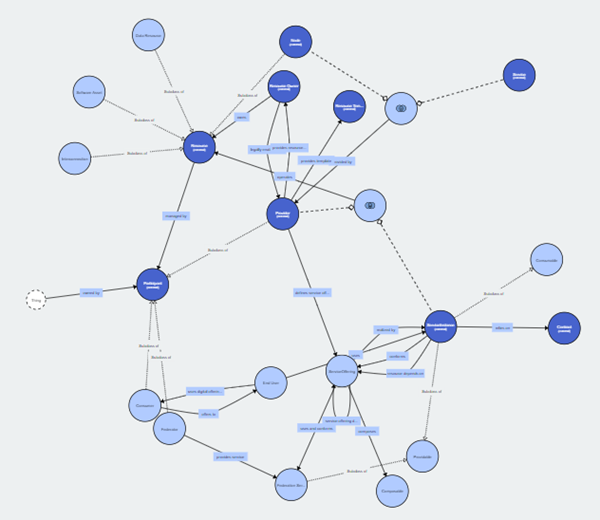
\includegraphics[width=0.7\linewidth]{introduction/figures/ontology_example.jpg}
   \end{center}
   \caption[Ontología: Ejemplo 1]
   {\footnotesize Ontología: Ejemplo 1}
   \label{fig:mufigure6}
\end{figure}

En la Figura 2, podemos ver una estructura de datos en la cual cada concepto está representado por un círculo, y entre ellos están conectados por diferentes tipos de líneas, para diferenciar las relaciones.

\begin{figure}[ht]
   \begin{center}
      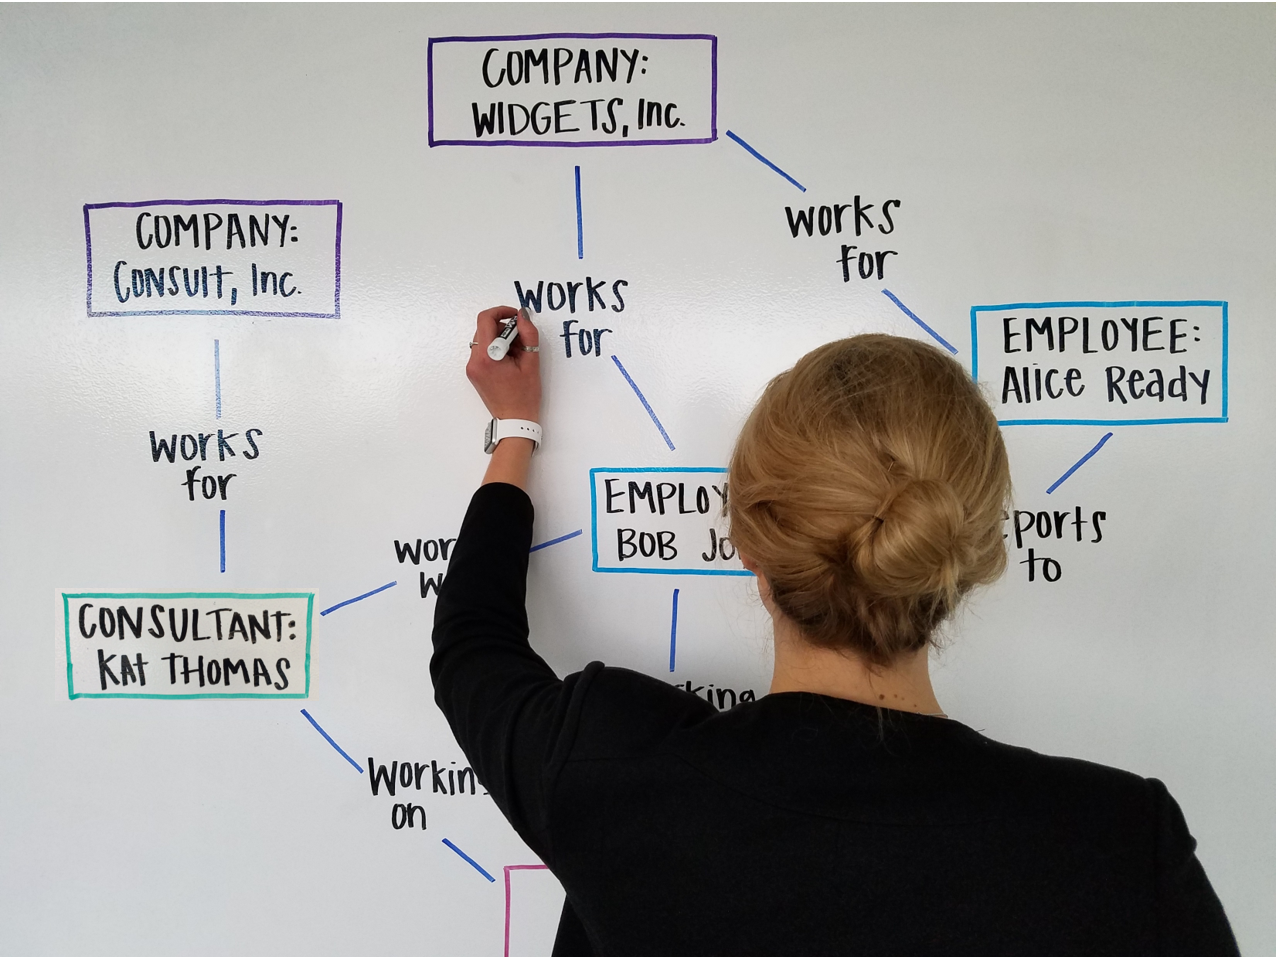
\includegraphics[width=0.7\linewidth]{introduction/figures/ontology_example_2.png}
   \end{center}
   \caption[Ontología: Ejemplo 2]
   {\footnotesize Ontología: Ejemplo 2}
   \label{fig:mufigure6}
\end{figure}

En la Figura 3, vemos como una empresa puede ser representada a través de ontologías al representar sus componentes como clases.

\begin{figure}[ht]
   \begin{center}
      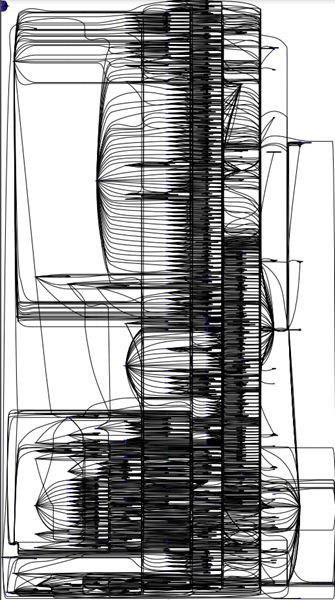
\includegraphics[width=0.4\linewidth]{introduction/figures/ontology_example_3.jpg}
   \end{center}
   \caption[Ontología: Ejemplo 3]
   {\footnotesize Ontología: Ejemplo 3}
   \label{fig:mufigure7}
\end{figure}

Para introducir de a poco la problématica que queremos enfrentar, podemos ver la Figura 4, que muestra qué tan compleja se puede ver una ontología si la cantidad de clases y relaciones incrementa demasiado.
Esta idea la iremos expandiendo un poco más en otras secciones.

\section{Gaia-X}

Gaia-X es una iniciativa que desarrolla, sobre la base de los valores europeos, una gobernanza digital que puede aplicarse a cualquier pila tecnológica existente de nube para obtener transparencia, controlabilidad, portabilidad e interoperabilidad entre datos y servicios. \cite[]{Gaiax}

\begin{figure}[ht]
   \begin{center}
      
\includegraphics[width=0.4\linewidth]{introduction/figures/gaia-x.png}
   \end{center}
   \caption[Logo de Gaia-X]
   {\footnotesize Logo de Gaia-X}
   \label{fig:mufigure7}
\end{figure}

Hoy en día, muchos negocios de pequeña y mediana dimensión desarrollan interfaces individualmente para cada cliente para el intercambio de informacion y la interoperabilidad de soluciones. Esto cuesta tiempo y dinero. Gaia-X busca proveer mecanismos comunes de intercambio de información que adhieran a las necesidades comunes de confianza.

En Europa, la adapcion de tecnologías de nube es solo del 26\%. Esto implica que la mayoría de la información y las aplicaciones son todavía inaccesibles e initercambiables. Gaia-X desarrollará una estructura de trabajo que le permita a la gente tomar decisiones informadas a la hora de intercambiar información. 

¿Por qué están relacionados este proyecto con las ontologías? La descripción de entidades ha sido siempre uno de los objetivos de la informática. En primer lugar, porque ayuda a comprender la entidad descrita, y después porque su análisis sintáctico permite aplicar reglas y construir funcionalidades.

El objetivo de la ontología es ser abierta y compartida: describe lo que son las cosas en general, no en un contexto específico. De este modo se simplifica el proceso de diseño de nuevas ontologías, ya que se puede recurrir a las existentes, y también se facilita la interacción con otras organizaciones, porque se utilizan las mismas ontologías.

Por último, y quizá el punto más crucial, la ontología puede ser analizada fácilmente por una máquina, lo que facilita el razonamiento. \cite[]{GaiaxOntology}

El desarrollo del proyecto Gaia-X naturalmente va a depender de las ontologías y los softwares requeridos, por esta razón tenemos que asegurarnos de contar con herramientas adecuadas.


\clearemptydoublepage
\mainmatter
\clearemptydoublepage
\chapter{Estado del Arte}
\chaptermark{Estado del Arte}

Organizar información a través de ontologías es muy común en diferentes ámbitos científicos como la biomedicina, informática, filosofía, etc.
Esto ha dado lugar a numerosas opciones de software dedicado a representar dichas ontologías \cite[]{ontologyEditors}. Estos editores se encargan de tareas como creación,
edición, visualización, exploración, \textit{debugging}, etc. Por estas razones, el desarrollo de una aplicación para trabajar con ontologías no es
una tarea sencilla, y requiere de mucho estudio y planeamiento, ya que todas tienen falencias y puntos débiles en distintas etapas del trabajo \cite[]{ontologyIssues}.

Todas las herramientas que podemos encontrar tienen la característica común de trabajar solo en el espacio bidimensional, como la inmensa mayoría de programas hoy en día.
Por esta razón, si queremos expandir el horizonte de la tecnología, debemos empezar a probar qué tan útil es la Realidad Extendida en diferentes ámbitos. En este caso,
vamos a tomar como referencia el software más utiizado con fines de visualización, llamado Protégé.

\begin{figure}[ht]
   \begin{center}
      
\includegraphics[width=0.7\linewidth]{chapter1/figures/protege.jpg}
   \end{center}
   \caption[Protégé Logo]
   {\footnotesize Protégé Logo}
   \label{fig:mufigure3}
\end{figure}

Es un editor de ontologías gratis y open-source, que provee un esquema de trabajo para construir sistemas inteligentes y se caracteriza
por brindar una útil interfaz de visualización, a diferencia de otros softwares de ontologías. Sin embargo, aprender a operar esta herramienta no es fácil
y requiere bastante tiempo y dedicación \cite[]{ontologyTutorial}.

El principal problema de este tipo de programas, es el rendimienot limitado en grandes ontologías. Aunque Protege es adecuado para la mayoría de las necesidades de modelado de ontologías, puede experimentar limitaciones de rendimiento al trabajar con ontologías muy grandes o complejas. En tales casos, los usuarios pueden encontrar que el rendimiento de la herramienta se ralentiza o que experimentan problemas de memoria.
Sumado al hecho de que compartir una ontología a través de imágenes o capturas de pantalla en un reporte, complica demasiado la interpretación y no se puede apreciar correctamente lo que se está representando.

\clearemptydoublepage
\clearemptydoublepage
\chapter{Trabajo Realizado}
\chaptermark{Trabajo Realizado}

En este capítulo intentaré explicar y mostrar los aspectos generales de las funciones que llegué a desarrollar durante mis prácticas.
Proporcionaré diagramas de datos y algunas imágenes que ayuden a entender la idea que hay detrás de muchas soluciones a los problemas a los que nos enfrentamos como equipo.

La información real del proyecto permanecerá oculta por cuestiones de confidencialidad, pero no afectará a la comprensión del trabajo.

\section{Planeación de Desarrollo}

\begin{figure}[ht]
    \begin{center}
       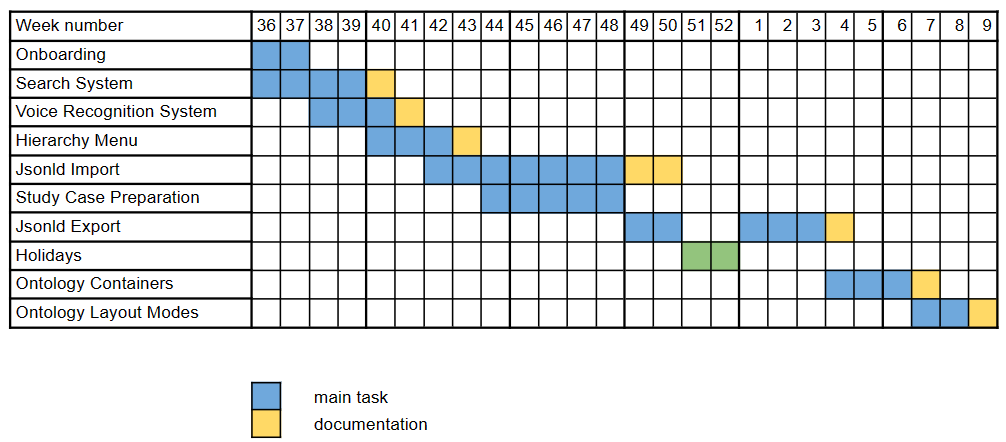
\includegraphics[width=1\linewidth]{chapter2/figures/gantt.png}
    \end{center}
    \caption[Planeacion de Desarrollo en Diagrama de Gantt]
    {\footnotesize Planeacion de Desarrollo en Diagrama de Gantt}
    \label{fig:mufigure3}
 \end{figure}

\section{Visualizador de Ontologías}

Esta aplicación tiene objetivos muy concretos. En primer lugar, integrarse al sistema y formato creado por Gaia-X, por lo tanto, debemos incorporar un método para leer los archivos provenientes de este proyecto.
Segundo, nos enfocaremos en tareas de visualización de ontologías y no tanto de creación o \textit{debugging}. Este último punto nos determina el tipo de herramientas a priorizar, como pueden ser métodos de filtrado de clases,
búsqueda, comparación de propiedades, manipulación de la apariencia de las ontologías, etc. Más adelante, una vez tengamos este punto cubierto, veremos qué podemos desarrollar para la edición de una ontología. Mientras tanto, debemos
asegurarnos de poder incorporar nuestra aplicación al conjunto de software disponible y asi utilizarla en conjunto con las opciones dedicadas a otras tareas.

La escena desarrollada se ve como en la Figura 2.2. Aquí podemos observar, desde el punto de vista del usuario, como se enfrentaría a un grupo de clases provenientes de 4 ontologías diferentes.

\begin{figure}[ht]
   \begin{center}
      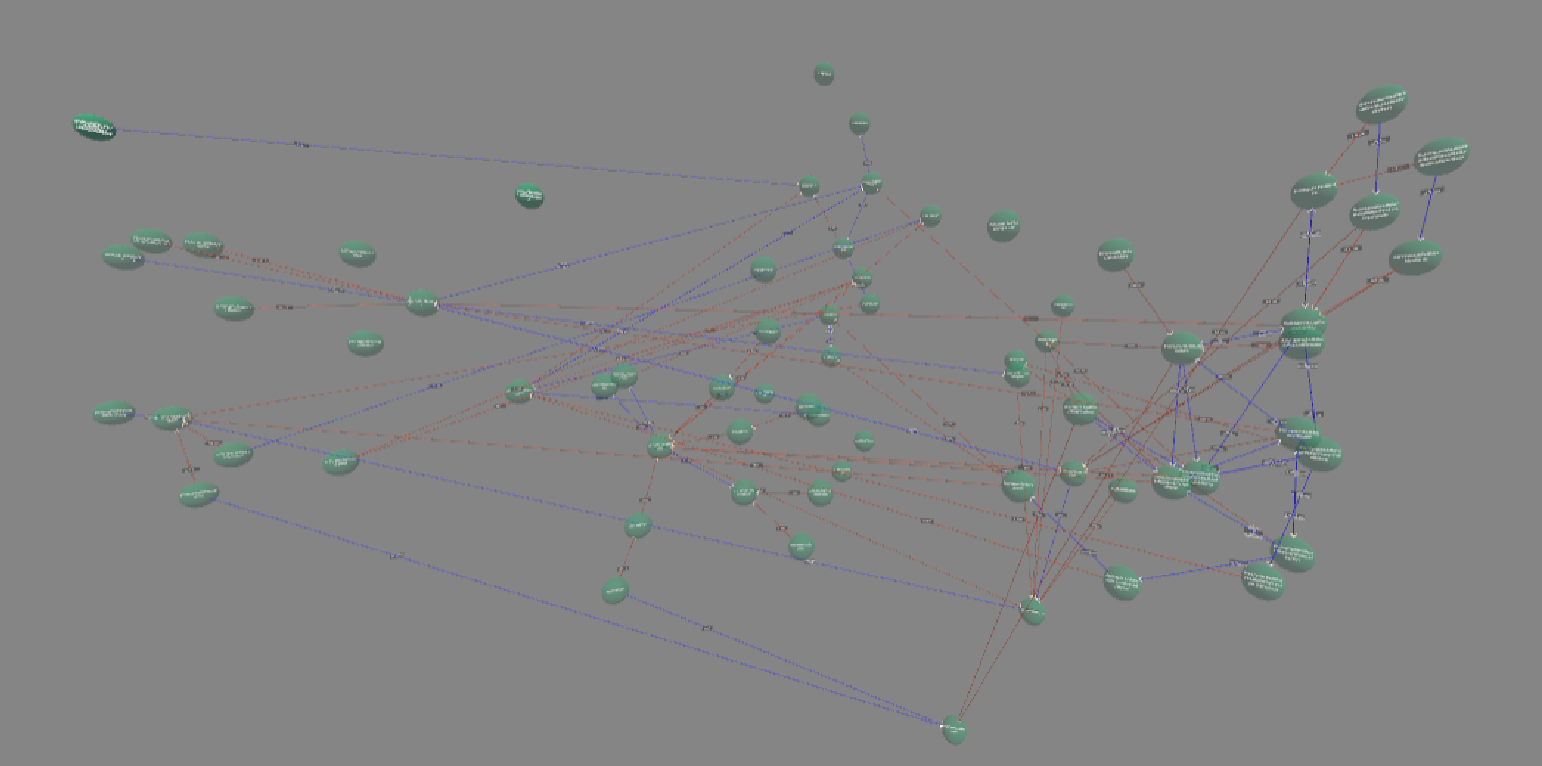
\includegraphics[width=0.7\linewidth]{chapter2/figures/ontology_project.png}
   \end{center}
   \caption[Escena desarrollada]
   {\footnotesize Escena desarrollada}
   \label{fig:mufigure9}
\end{figure}

Cada clase está representada por una instanciación de la clase \textit{Bubble} y se conecta a otras clases a través de dos tipos de conexiones diferentes:
\begin{itemize}
   \item Herencia: en el que se especifica que una clase es subclase de otra de mayor jerarquía. (conexión naranja)
   \item Relación específica: una conexión que incluye una etiqueta de texto para especificar de qué manera se conectan dichas clases. (conexión azul) 
\end{itemize}

\section{Software de Desarrollo}

El proyecto se desarrolló con Unity (versión 2021.3.23f1). Se trata de una plataforma de desarrollo de juegos potente y versátil que ha revolucionado la forma de crear juegos, desde proyectos independientes hasta grandes éxitos de taquilla. Con Unity, los desarrolladores pueden diseñar, crear e implantar juegos de alta calidad en multitud de plataformas, como dispositivos móviles, consolas y PC. Su interfaz fácil de usar y su amplia biblioteca de recursos lo hacen accesible tanto para los profesionales experimentados como para los recién llegados al desarrollo de juegos.

Uno de los aspectos más atractivos de Unity es su capacidad para facilitar la creación rápida de prototipos y la iteración. Los desarrolladores pueden dar vida rápidamente a sus ideas, probar mecánicas de juego y perfeccionar sus creaciones en tiempo real. Esta agilidad no sólo acelera el proceso de desarrollo, sino que también permite una mayor creatividad y experimentación.

Además, Unity ofrece un vasto ecosistema de activos, plugins y apoyo de la comunidad, lo que permite a los desarrolladores ampliar la funcionalidad de la plataforma y colaborar con otros creadores. Desde activos y scripts prefabricados hasta técnicas avanzadas de renderizado y algoritmos de inteligencia artificial, Unity proporciona una gran cantidad de recursos para agilizar el desarrollo y mejorar la calidad de los juegos.

\subsection{OpenXR}

Para conectar Unity con el casco de realidad virtual, optamos por OpenXR, un estándar abierto que pretende agilizar el desarrollo de aplicaciones de realidad virtual proporcionando una API común para interactuar con el hardware de realidad virtual. Desarrollado por Khronos Group, un consorcio industrial centrado en el desarrollo de estándares abiertos para gráficos y computación paralela, OpenXR pretende abordar la fragmentación del ecosistema de realidad virtual y realidad aumentada permitiendo a los desarrolladores crear aplicaciones compatibles con una amplia gama de dispositivos, plataformas y entornos de ejecución. \cite[]{OpenXR}

\begin{figure}[ht]
   \begin{center}
      
\includegraphics[width=0.4\linewidth]{chapter2/figures/OpenXR_logo.png}
   \end{center}
   \caption[OpenXR logo]
   {\footnotesize OpenXR logo}
   \label{fig:mufigure8}
\end{figure}

Proporciona un conjunto de API estándar para funciones como el renderizado, el manejo de entradas, el seguimiento y la interacción, lo que permite a los desarrolladores acceder y controlar las capacidades de los dispositivos de hardware de realidad virtual y realidad aumentada de forma coherente e independiente de la plataforma.
Esto fue de enorme relevancia, debido a que en nuestro departamento disponíamos de diferentes headsets para desarrollo y presentaciones, como el HTC Vive Pro, HTC Focus y Meta Quest 2, por lo que la estandarización fue crucial para la mejora consistente en nuestro proyecto.

\subsection{XR Interaction Toolkit}

Otro elemento central de este proyecto fue el uso del \textit{XR Interaction Toolkit} de Unity, que permite todo tipo de interacciones entre el jugador y el entorno.

El paquete XR Interaction Toolkit es un sistema de interacción de alto nivel basado en componentes para crear experiencias de realidad virtual y realidad aumentada. Proporciona un marco que hace que las interacciones 3D y de interfaz de usuario estén disponibles a partir de eventos de entrada de Unity. El núcleo de este sistema es un conjunto de componentes base \textit{Interactor} e \textit{Interactable}, y un \textit{Interaction Manager} que une estos dos tipos de componentes. \cite[]{XRInteraction}

Si observamos el conjunto de Figuras 2.4, vemos algunos ejemplos de interacciones que podemos utilizar gracias a esta kit de herramientas. Con el puntero raycast, manteniendo el click presionado mientras apuntamos a una burbuja, podemos desplazarla en el espacio como queramos. Ese mismo puntero nos permite teletransportarnos a una burbuja deseada si movemos el joystic hacia adelante al apuntarle. También podemos interactuar con elementos de UI como botones e imágenes. 

\begin{figure}[ht]
   \centering
   \begin{subfigure}{0.45\textwidth}
       \centering
       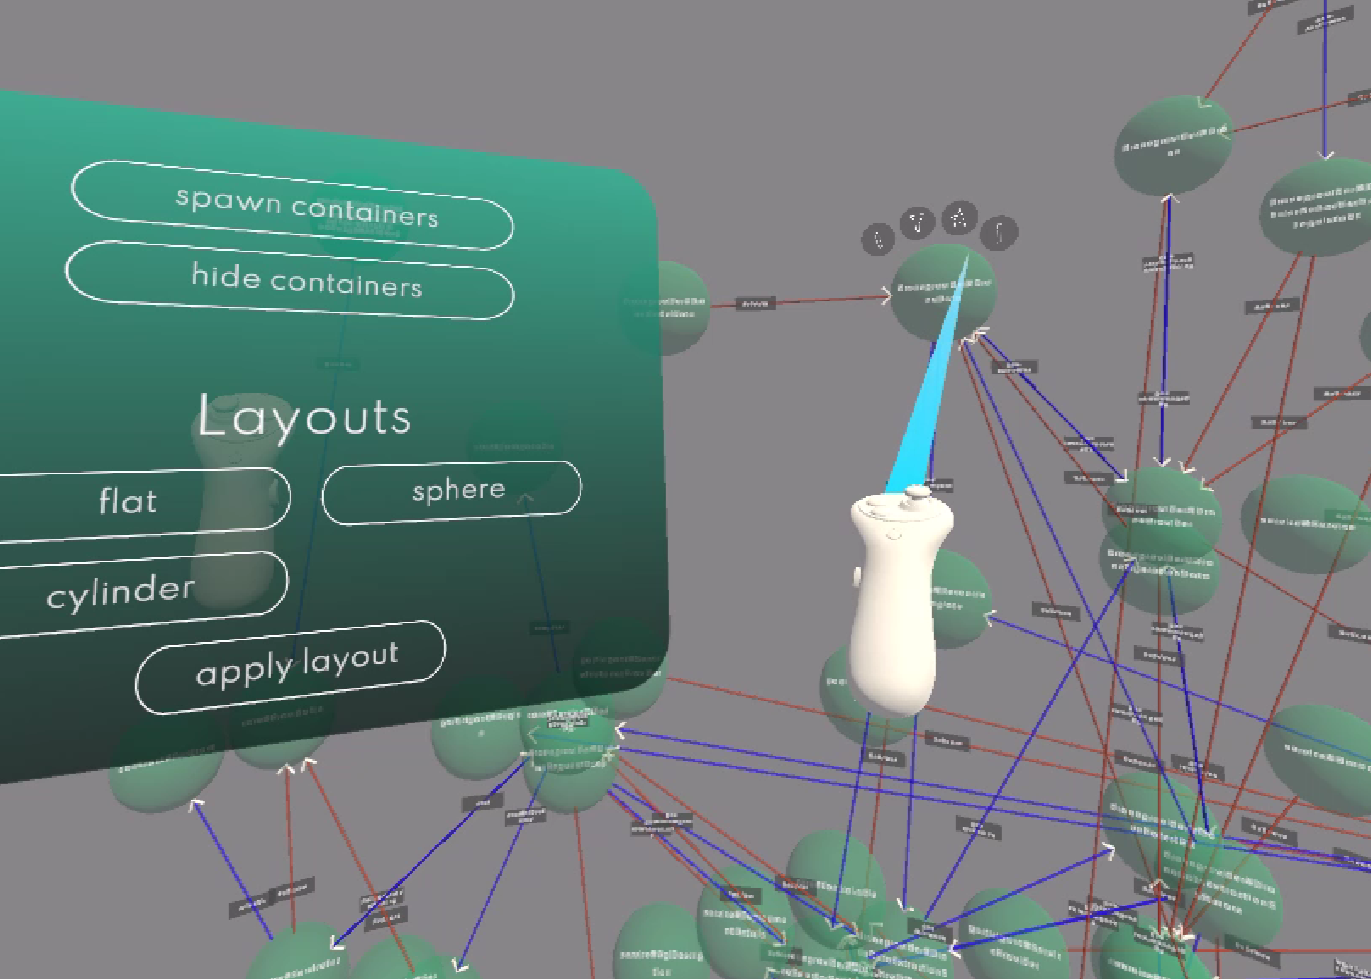
\includegraphics[width=\textwidth]{chapter2/figures/raycast.png}
       \caption{Puntero Raycast}
   \end{subfigure}
   \hfill
   \begin{subfigure}{0.45\textwidth}
       \centering
       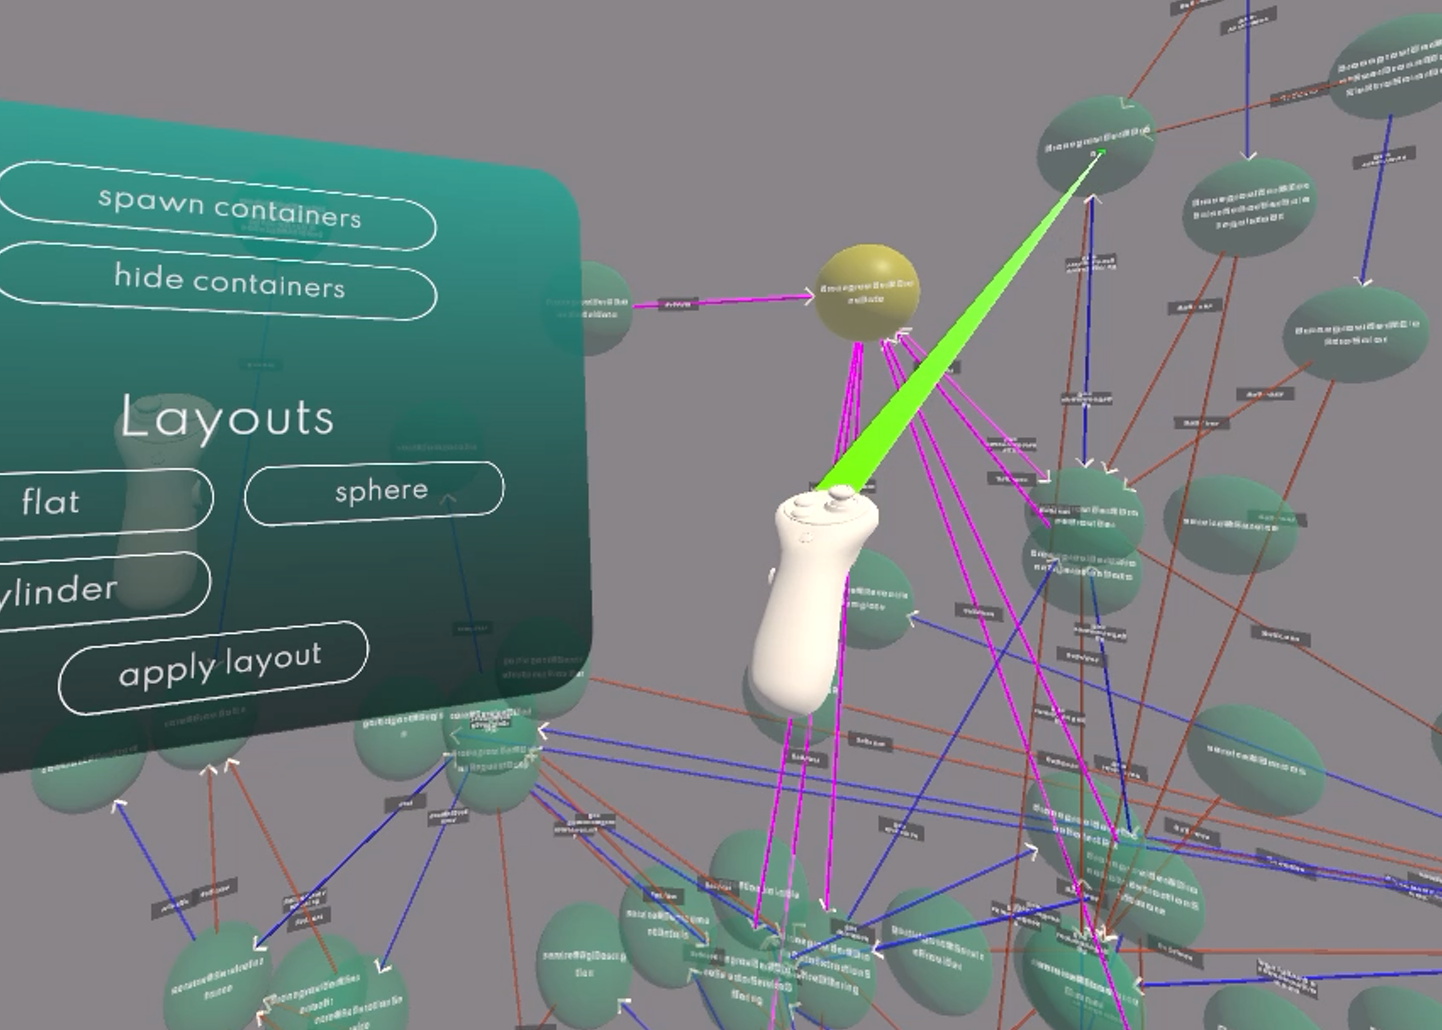
\includegraphics[width=\textwidth]{chapter2/figures/teleport.png}
       \caption{Teletransportación}
   \end{subfigure}
   \\
   \begin{subfigure}{0.45\textwidth}
       \centering
       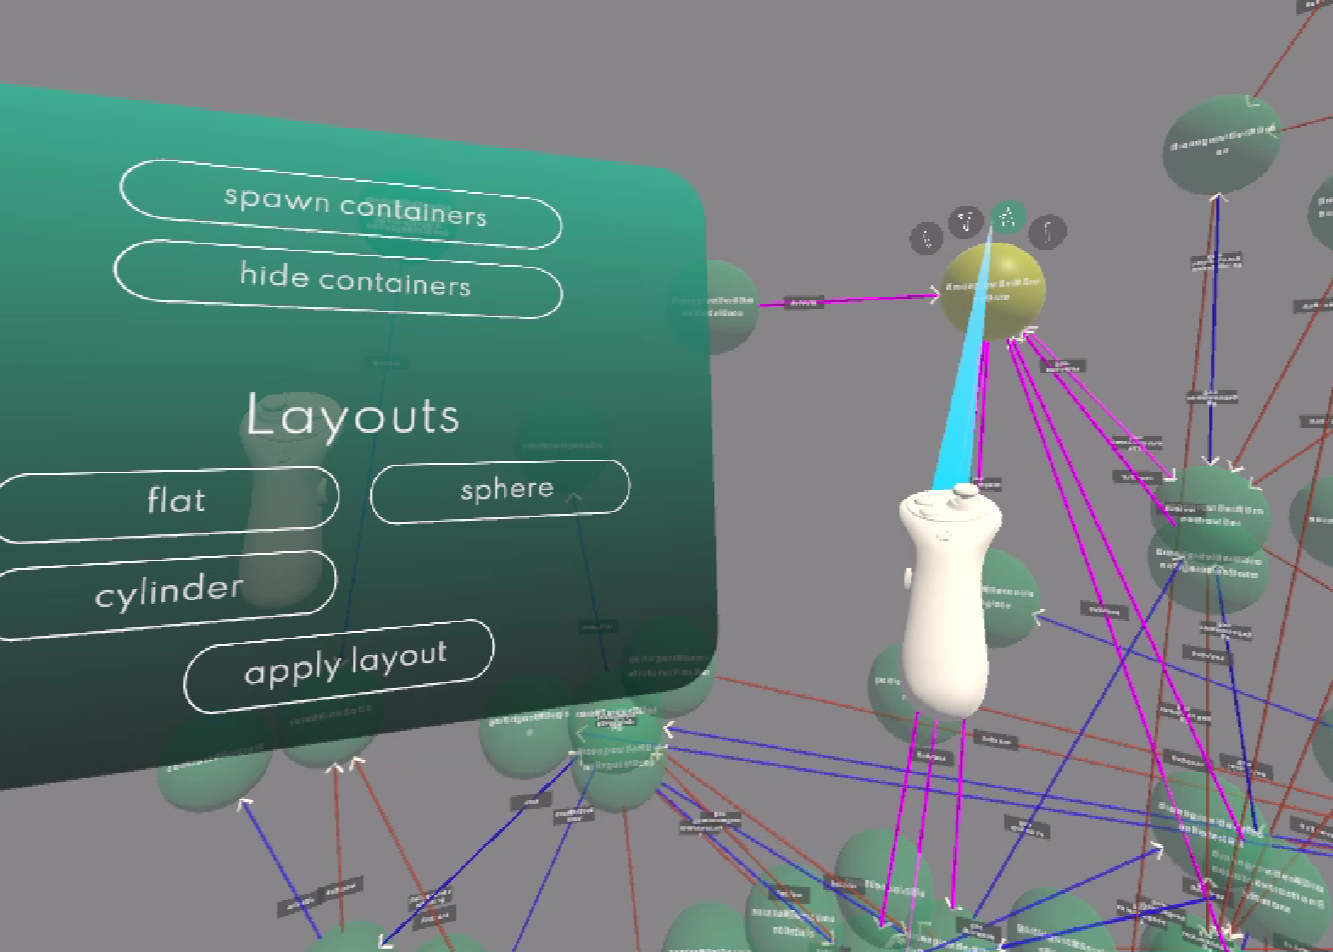
\includegraphics[width=\textwidth]{chapter2/figures/highlight.png}
       \caption{Interacciones con UI}
   \end{subfigure}
   \caption{Interaccioes del Toolkit}
   \label{fig:subfigures}
\end{figure}

\section{Funciones Desarrolladas}

\subsection{Sistema de Búsqueda}

Implementar un sistema de búsqueda es casi obligatorio a la hora de crear un software de datos e información. Siempre necesitamos comprobar la existencia de clases y en la mayoría de los casos los resultados de búsqueda tienen también una funcionalidad asociada. En nuestro caso optamos por 2 diferentes, que pueden ser habilitadas desde el inspector de Unity: resaltar la burbuja elegida o teletransportarse a ella si se desea. Esto demostró ser extremadamente útil y escala muy bien si la cantidad de clases aumenta.
Para cualquiera de estas funcionalidades, necesitábamos asociar cada resultado de búsqueda a la burbuja correcta, para que podamos encontrar la referencia a los métodos de la burbuja. Resaltar es sólo cambiar el color del material mientras que la teletransportación reposiciona al jugador y lo orienta hacia la burbuja en cuestión.

El proceso de búsqueda es manejado por el \textit{Search Manager} y su componente principal \textit{SearchScript.cs}. Está conectado al campo de entrada de búsqueda y llama al método Search() cada vez que hay un cambio en el texto de entrada. Dicho script contiene una lista \textit{List<GameObject>Elements} que contiene todas las clases de la escena. Esta es llenada al crear las burbujas para las clases extraidas de un archivo, pero eso lo veremos en otra sección.

Cuando hay una coincidencia entre el texto de entrada y el nombre de cualquier burbuja, creamos botones dentro de un panel y los referenciamos a su burbuja correspondiente, de modo que podemos llamar a un método específico al pulsar sobre él.

Los métodos son los siguientes:
\begin{itemize}
   \item Search: este es el método de callback cada vez que se modifica el campo de entrada de texto. Se encarga de comparar el texto ingresado con los nombres de las clases de la escena y crear una lista de resultados compuesta por referencias a las burbujas correspondientes.
   \item DeleteButtons: cada vez que ingresamos una letra, los resultados cambian. Por esta razón, debemos borrar los botones de los resultados de la búsqueda anterior.
   \item CreateButtons: instancia un botón por cada burbuja que haya dentro de la lista de resultados y realiza las conexiones necesarias para las funciones de callback de cada botón, ya se teletransportar o resaltar. También resalta el texto dle botón que coincida con la búsqueda.
   \item ResetSearch: vacía el campo de entrada para cuando se complete una función de callback y así se resetea el sistema.
   \item UpdateResultsButton: es un sistema de \textit{flag} para determinar el mensaje de estado de búsqueda. Este es transmitido al usuario a través de un cuadro de texto.
\end{itemize}

\begin{figure}[ht]
   \begin{center}
      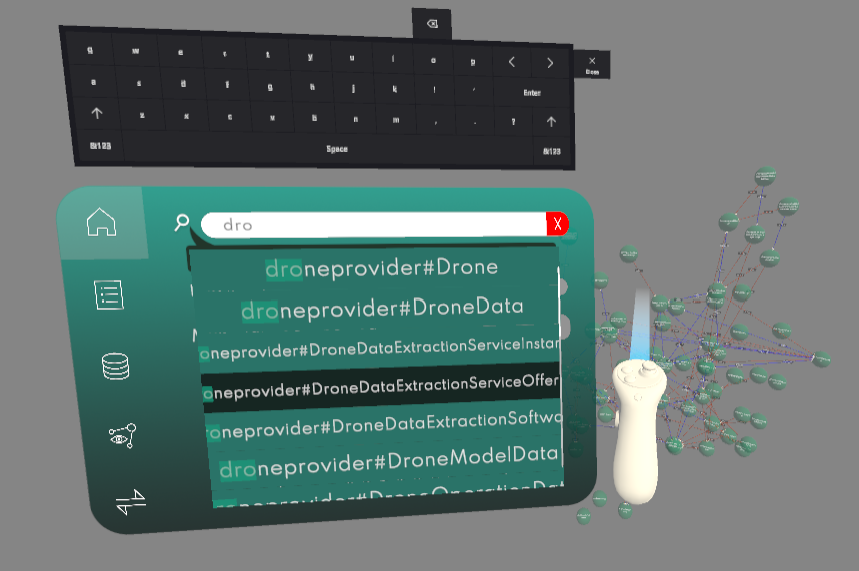
\includegraphics[width=0.7\linewidth]{chapter2/figures/searchtool.png}
   \end{center}
   \caption[Búsqueda de clases y resultados]
   {\footnotesize Búsqueda de clases y resultados}
   \label{fig:mufigure10}
\end{figure}

Esta herramienta se incorpora al menú de la mano, que se acopla al mando de la mano izquierda en la simulación, e interactuamos con él con el raycast del mando de la mano derecha. Esta es una forma muy intuitiva y frecuente de añadir un menú en las simulaciones de RV.

Añadimos un teclado que obtuvimos de un proyecto de código abierto en Github y funcionó perfectamente desde el principio. \cite[]{Keyboard}

La figura 2.6 ilustra un poco el funcionamiento del proceso de búsqueda. Incluye el Reconocimiento de Voz explicado en la sección siguiente.

\begin{figure}[ht]
   \begin{center}
      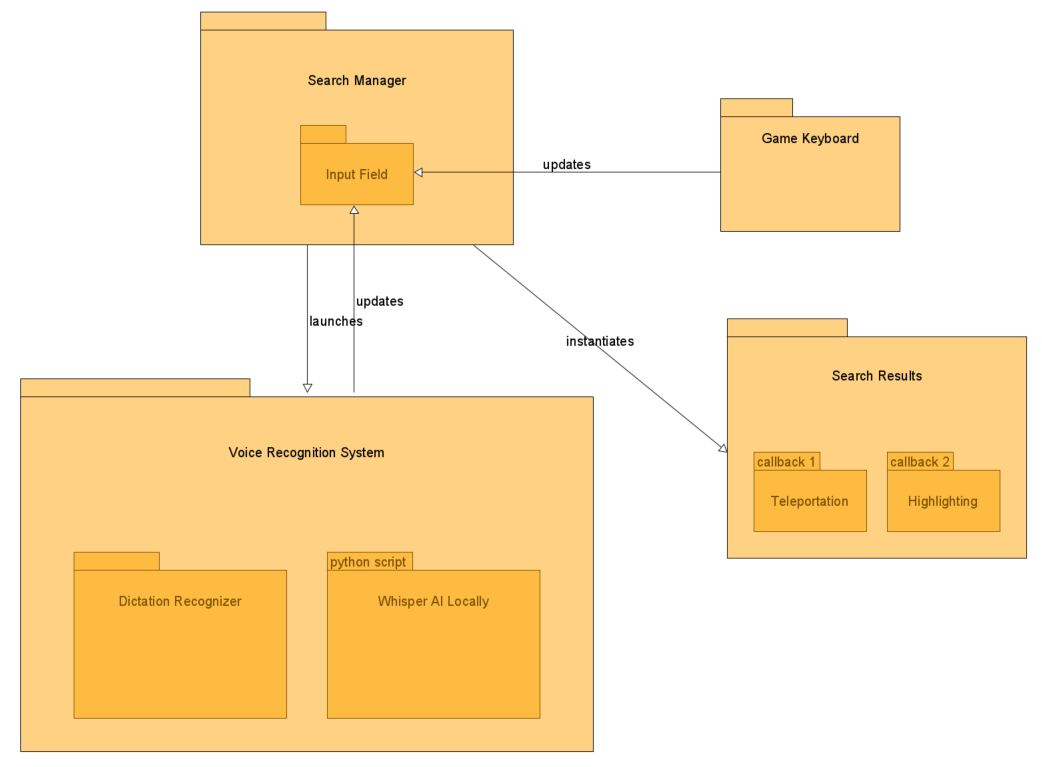
\includegraphics[width=1\linewidth]{chapter2/figures/searchsystem.png}
   \end{center}
   \caption[Diagrama de Paquetes del Sistema de Búsqueda]
   {\footnotesize Diagrama de Paquetes del Sistema de Búsqueda}
   \label{fig:mufigure10}
\end{figure}

\subsection{Sistema de Reconocimiento de Voz}

Para complementar el Sistema de Búsqueda, pensamos que sería buena idea implementar un Sistema de Reconocimiento de Voz con IA para reducir los tiempos de tecleo. La principal limitación era que para conseguirlo necesitábamos una herramienta offline, de forma que el proyecto no dependiera de la conexión a internet y los datos se mantuvieran seguros y confidenciales.
Esto era bastante difícil dado que los mejores sistemas gratuitos de reconocimiento de voz requieren conexión o si no, son servicios de pago.

Después de investigar un poco encontré algunas alternativas, pero necesitaba probarlas y ver cuál funcionaba mejor.
\begin{itemize}
   \item \textbf{Servicios fuera de línea:}
   \begin{itemize}
      \item \textbf{DeepSpeech:}
      Motor Speech-To-Text de código abierto, que utiliza un modelo entrenado mediante técnicas de aprendizaje automático basado en el trabajo de investigación Deep Speech de Baidu. El proyecto no ha recibido actualizaciones desde 2020 y no hay soporte para las últimas versiones de python, por lo que para usarlo es necesario utilizar una herramienta como win-pyenv para gestionar versiones antiguas. Siguiendo el único tutorial online, conseguí instalarlo pero el reconocimiento no fue bueno, alrededor de un 20\% y un 30\% de efectividad.
      \item \textbf{Vosk:}
      También es un kit de herramientas offline pero con soporte en diferentes idiomas. En su página web principal ofrecen un ejemplo de Unity, pero los resultados no fueron buenos y no se reconoció ninguna palabra.
      \item \textbf{Unity Keyword Recognizer:}
      Haciendo uso del servicio de reconocimiento de voz de Windows, podemos reconocer palabras y compararlas con comandos de la lista para activar eventos específicos. Inconveniente: hay que añadir manualmente cada comando a la lista y la llamada de retorno correspondiente.
      \item \textbf{WhisperAI:}
      Normalmente WhisperAI requiere una API y pagas cada vez que lo usas, pero también puedes instalarlo localmente usando la librería pip para python.
      \item \textbf{Undertone:}
      Un activo de pago en Unity Store que también funciona sin conexión con WhisperAI.   \end{itemize}
   \item \textbf{Servicios en línea:}
   \begin{itemize}
      \item \textbf{Unity Dictation Recognizer:}
      Funciona igual que el Reconocedor de Palabras Clave pero para identificar frases aleatorias necesitamos conexión a internet. Funciona bastante bien y reconoce los idiomas añadidos en la configuración de Windows del PC.
      \item \textbf{Hugging Face:}
      Es una IA online gratuita que proporciona una API con Unity y se encarga del reconocimiento de voz.
      \item \textbf{Recognissimo:}
      Es un activo de pago de Unity que también se encarga del reconocimiento de voz. Técnicamente está basado en el sistema Vosk.
   \end{itemize}
\end{itemize}

Habiéndolo consultado con mi equipo y mi supervisor, decidimos que implementaríamos la versión offline de WhisperAI y también probaríamos el Reconocedor de Dictados de Unity, dado que depende de Unity y Windows y usar la conexión a internet para eso era aceptable.
El sistema de búsqueda funciona de la misma manera, sólo estamos cambiando el método de entrada.

DictationRecognizer escucha la entrada de voz y trata de determinar qué frase fue pronunciada. \cite[]{DicationRecognizer}

Los usuarios pueden registrarse y escuchar los eventos de hipótesis y frase completada. Los métodos Start() y Stop() activan y desactivan respectivamente el reconocimiento del dictado. Una vez que se ha terminado con el reconocedor, debe ser desechado utilizando el método Dispose() para liberar los recursos que utiliza. Liberará estos recursos automáticamente durante la recolección de basura con un coste adicional de rendimiento si no se liberan antes.

La versión offline de WhisperAI fue muy interesante de usar ya que sólo puede leer archivos de audio y no voz en tiempo real. \cite[]{WhisperAI}

Esto añadía un nuevo paso en el proceso de reconocimiento ya que primero teníamos que grabar la voz y luego interpretarla con la librería instalada.
Desarrollé un script en Python que era llamado desde Unity cuando queríamos buscar algo por voz, y primero registraría la voz en un archivo, luego reconocería el texto en él y lo enviaría de vuelta a Unity abriendo un proceso e imprimiendo en él.
Unity estaría escuchando cualquier dato de entrada del proceso abierto después de llamar al script de python. Lo que era realmente interesante era que podíamos seleccionar el tamaño del modelo de entrenamiento, por lo que podíamos optimizar los recursos u optar por un mejor reconocimiento si lo deseábamos. Ver Figura 2.7.

\begin{figure}[ht]
   \begin{center}
      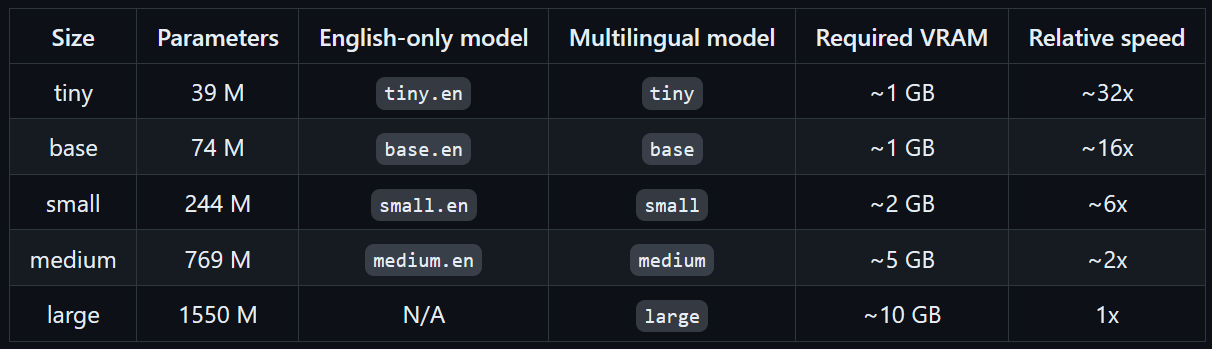
\includegraphics[width=0.85\linewidth]{chapter2/figures/whisperai.png}
   \end{center}
   \caption[Modelos de entrenamiento de Whisper AI]
   {\footnotesize Modelos de entrenamiento de Whisper AI}
   \label{fig:mufigure11}
\end{figure}

\subsection{Menú Jerárquico}

Esta característica fue desarrollada al principio de mi pasantía y en ese momento las ontologías eran diferentes a las que estamos usando ahora, por lo que esta desactualizada y requiere ser reestructurada para ser agregada al formato actual del proyecto.

La idea era tener una pestaña en el menú de mano donde pudiéramos ver rápidamente qué clases había en la escena según su nivel en la ontología. La inspiración para esto fue la interfaz del sistema de carpetas del Explorador de Windows. Vemos una carpeta y, al hacer clic en ella, expandimos el contenido que hay dentro y vemos las subcarpetas.
Así podemos navegar por nuestro sistema de datos y explorar todo lo que hay dentro. Esto era muy similar a nuestra antigua estructura ontológica, ya que teníamos un objeto Raíz y a partir de él empezábamos a conectar clases, de forma que cada una de ellas estaba conectada de alguna manera a ese objeto raíz.
Esto significaba que podíamos hacer clic y expandir una clase, para ver qué clases derivaban de ella, según su nivel en la ontología. En la Figura 2.8, podemos ver una ilustración de como sería este funcionamiento.

\begin{figure}[ht]
   \begin{center}
      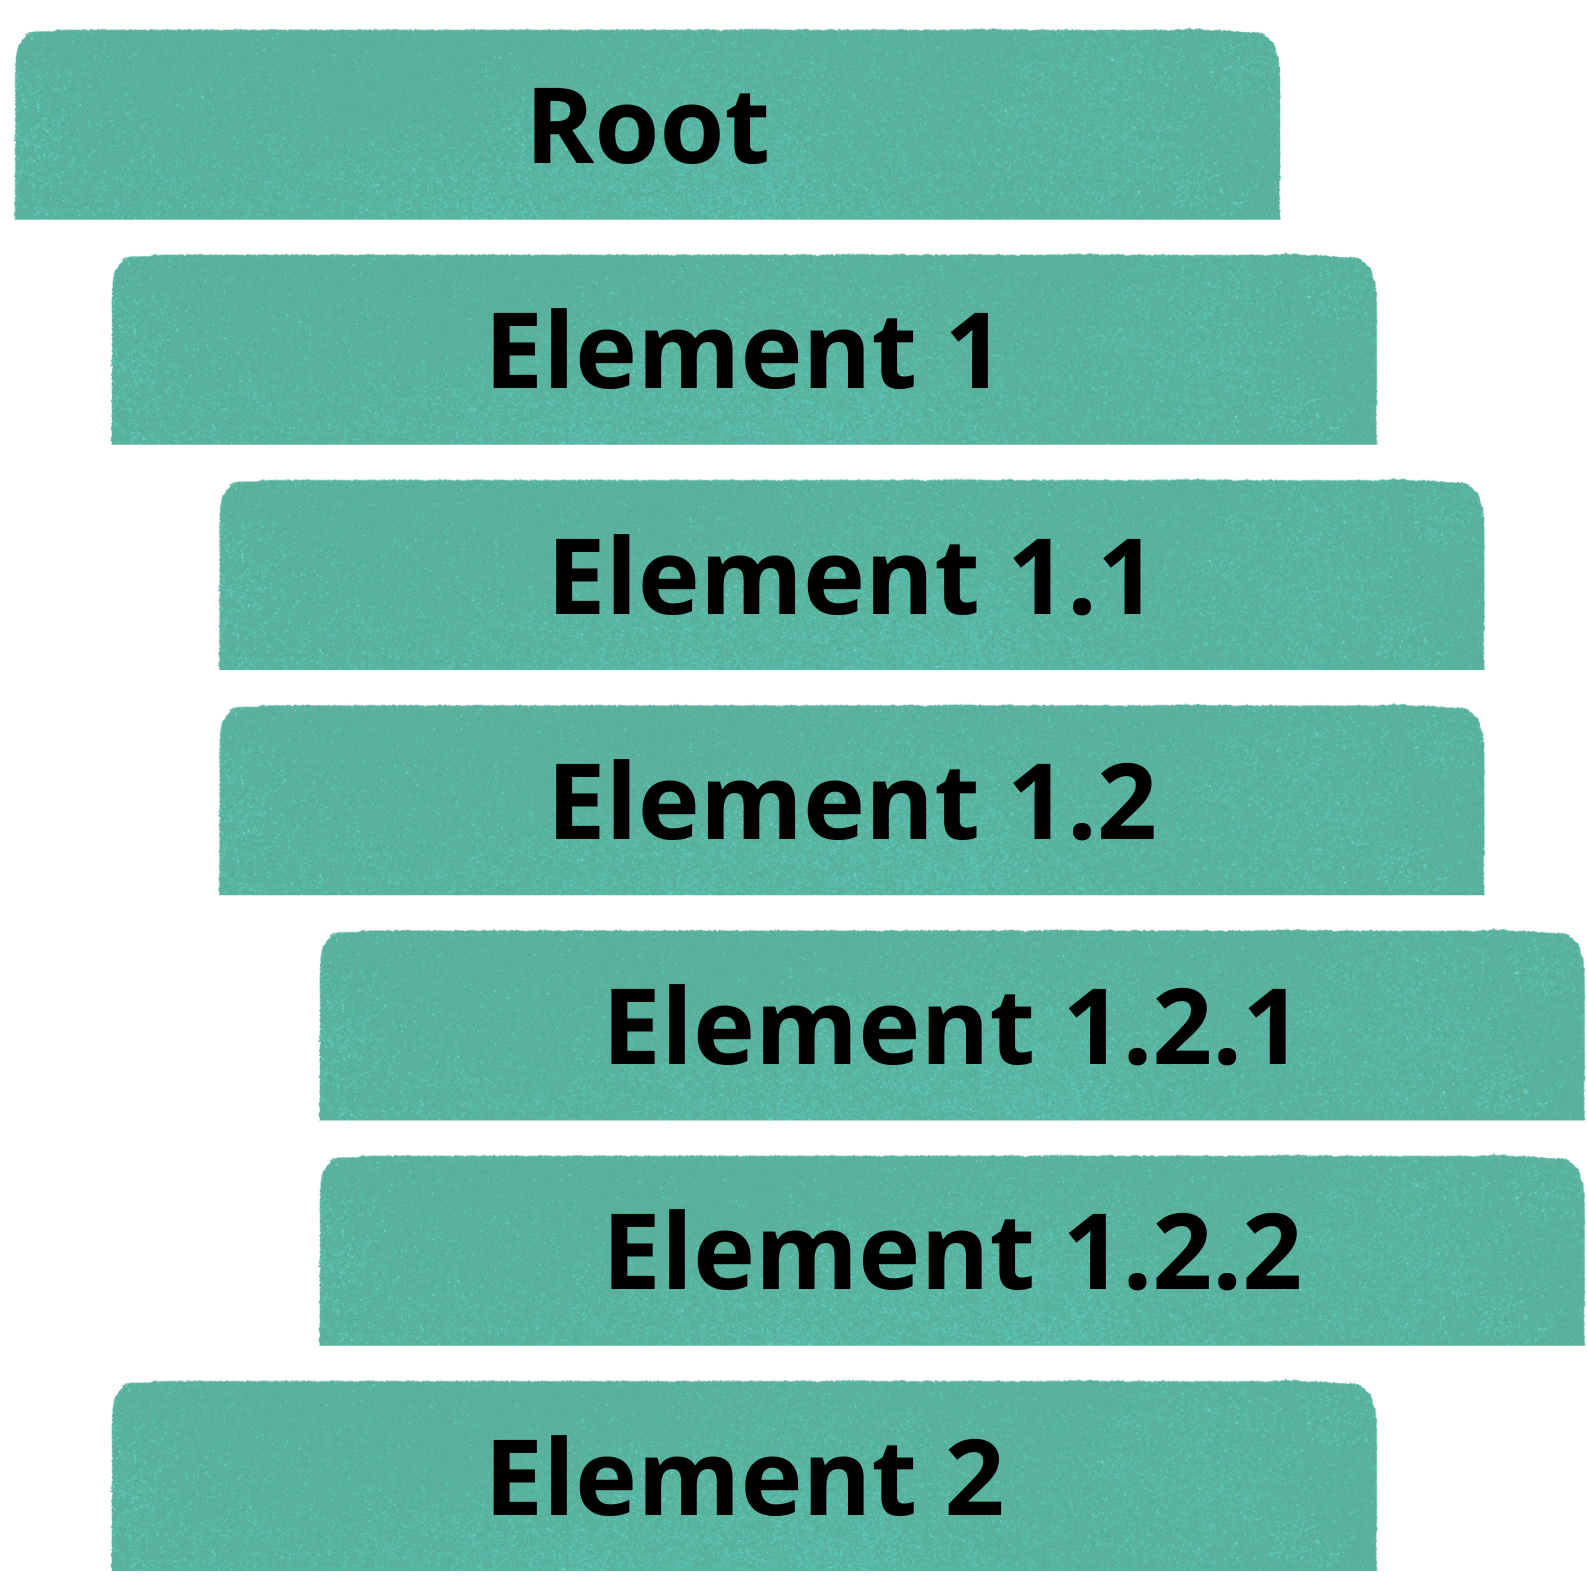
\includegraphics[width=0.6\linewidth]{chapter2/figures/hierarchy.png}
   \end{center}
   \caption[Ilustración gráfica de funcionamiento]
   {\footnotesize Ilustración gráfica de funcionamiento}
   \label{fig:mufigure11}
\end{figure}

La herramienta estaba implementada y funcionaba correctamente, y cada botón del menú también hacía referencia a las burbujas correspondientes, por lo que también teníamos funcionalidades de resaltado/teleportado asociadas a ellas. Todo esto cambió cuando empezamos a importar ontologías desde ficheros jsonld y el concepto de objeto raíz dejó de ser

\subsection{Importación desde archivos Jsonld}

Como he mencionado antes, esta simulación depende del Ontology Manager para cargar y guardar ontologías en archivos json, pero queremos ser capaces de leer información de Gaia-X y mostrarla en la escena para operar con ella. Después, deberíamos poder guardarla en un archivo similar y visualizarla en cualquier herramienta 2D y ver las modificaciones que hemos hecho.
Para esto necesitamos un Parser jsonld, para interpretar la información de Gaia-X y crear un archivo json que sea legible desde nuestro proyecto. Para ello hemos utilizado el paquete Newtonsoft Json Unity que nos ha facilitado mucho la tarea. \cite[]{json} 

El proceso de conversión es el resultado de un cuidadoso estudio por lo que necesita una explicación clara.
Primero descargamos el archivo JsonLD de la página web de la ontología Gaia-X en el estándar que han creado. Esta información luego pasa por dos procesos dentro de la escena Unity. El primero es un Parser para traducir el contenido y los datos a un formato estructurado con los valores que necesitamos para crear el objeto 3D en la escena. Esto incluye:

\begin{itemize}
   \item ID numérico único del juego
   \item Tipo de burbuja ( \textbf{Class} / Propiedad / Instancia )
   \item Nombre de la burbuja
   \item Posición 3D ( importada de otro archivo )
   \item Burbujas Poseídas
   \item Burbujas poseídas
   \item Heredado de Burbujas
   \item Heredado de Burbujas
\end{itemize}

Esta es toda la información que utilizamos para crear una Burbuja en la escena, por lo que es importante que no olvidemos ninguna de ellas en el proceso de parseo.
Este primer proceso se lleva a cabo en el momento de Inicio de la simulación pero esto puede ser cambiado a otro momento, como un menú de botones para importar ontologías específicas. De esta forma creamos un nuevo fichero que puede ser elegido para importar desde el Menú de Mano en la escena.
\begin{figure}[ht]
   \begin{center}
      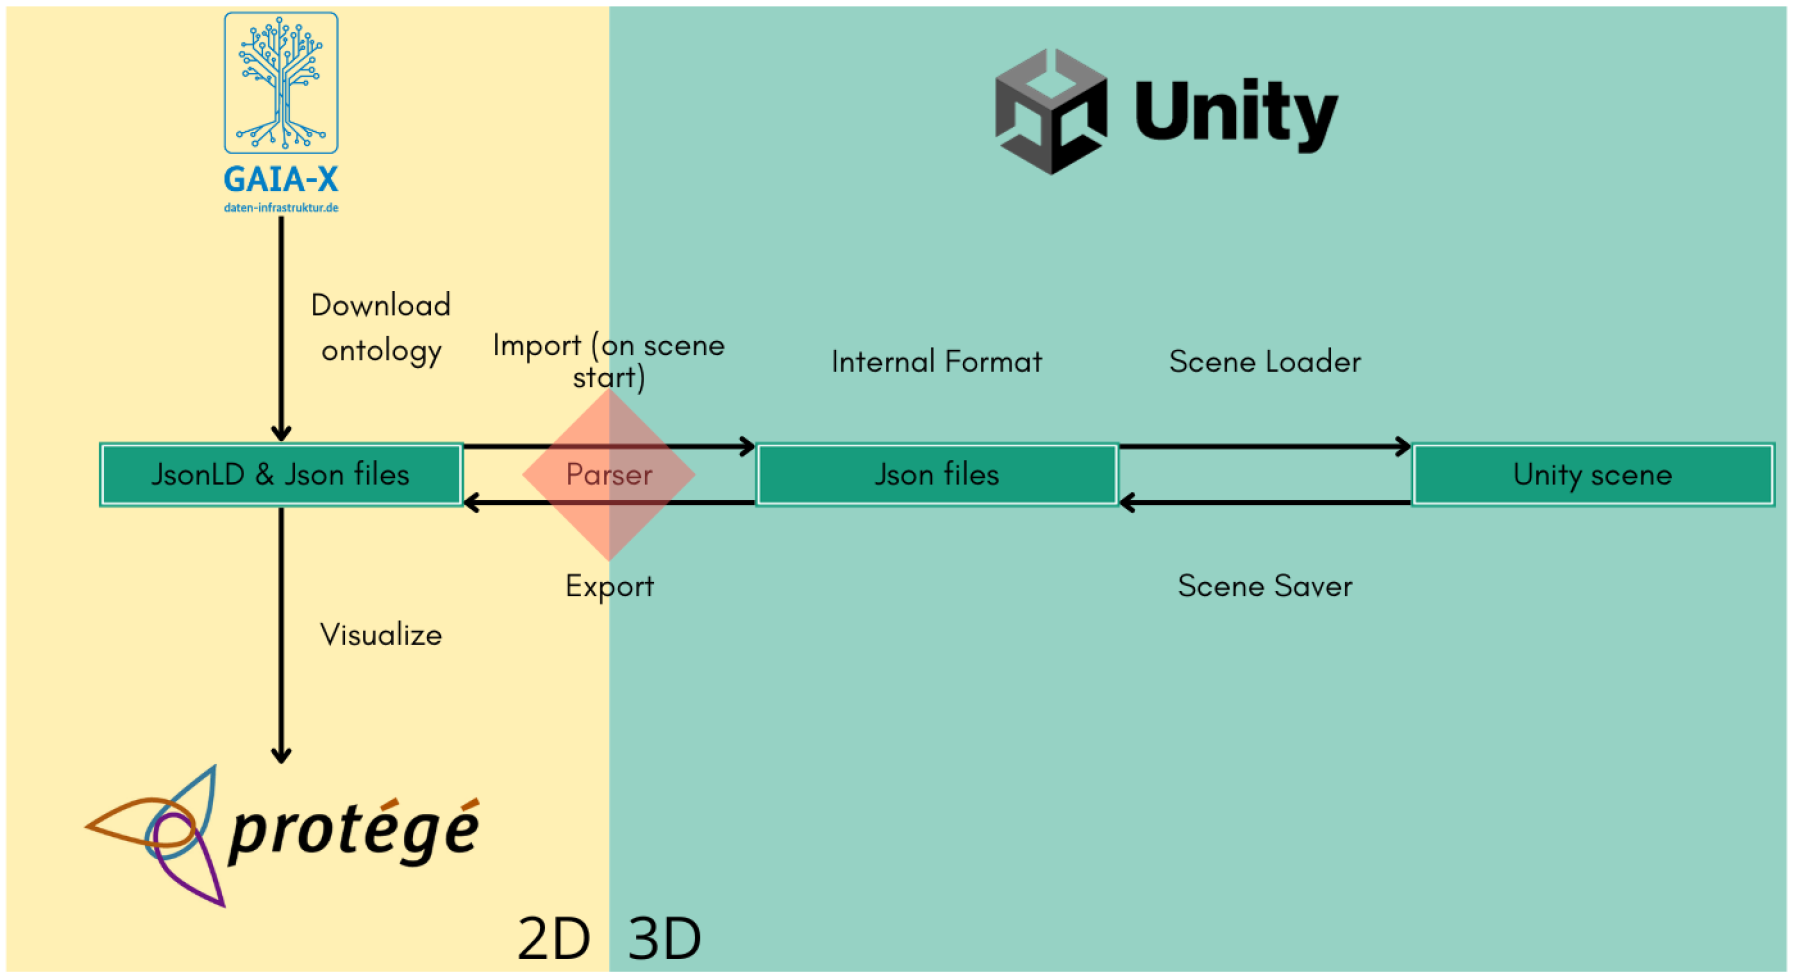
\includegraphics[width=0.85\linewidth]{chapter2/figures/importexport.png}
   \end{center}
   \caption[Import/Export process]
   {\footnotesize Import/Export process diagram}
   \label{fig:mufigure12}
\end{figure}

La forma en que filtramos la información es con una lista de condiciones if que comprueban la existencia de diferentes claves o propiedades json que nos guían y nos dicen qué información coger y cuál dejar, ya que el fichero jsonld contiene mucha información que no vamos a utilizar en nuestra escena, pero que necesitamos conservar para cuando exportemos la escena no perder ningún dato en el proceso.

A partir de los archivos jsonld que hemos descargado, buscamos en primer lugar objetos de dos tipos diferentes: Clases ("owl\#Class") y Conexiones ("owl\#ObjectProperty"). Analizaremos la información y almacenaremos las dos versiones de cada tipo en cuatro listas diferentes más una lista extra para almacenar toda la información no analizada que necesitaremos para el proceso de exportación. Con esa información, completaremos las listas de nuestro archivojson con las burbujas de propiedad y las subclases.

Para explicar cómo funciona la herramienta de importación, será más fácil si utilizamos un ejemplo de la lista de clases convertidas. También podemos ver el código 2.2 del apéndice.

\begin{figure}[ht]
   \begin{center}
      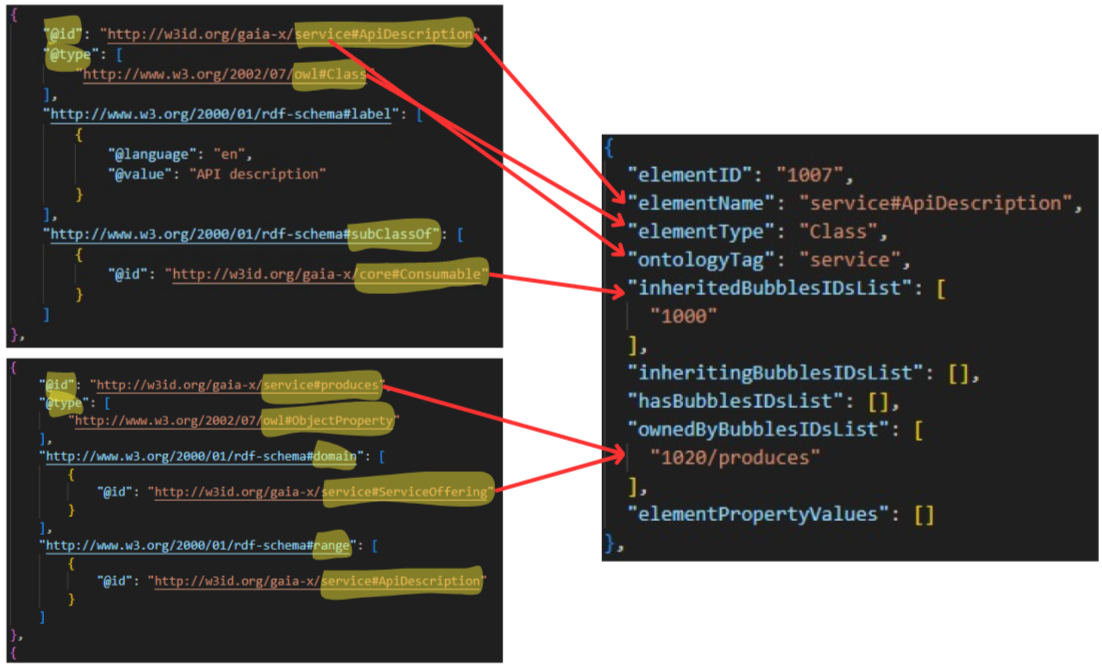
\includegraphics[width=0.9\linewidth]{chapter2/figures/parser.png}
   \end{center}
   \caption[Conversión de clase y conexión a formato interno]
   {\footnotesize Conversión de clase y conexión a formato interno}
   \label{fig:mufigure13}
\end{figure}

Cuando encontramos una clase, tenemos que deshacernos de la url en el id y quedarnos con el nombre real de la clase y la ontología a la que pertenece y asignarle un ID de objeto de juego único.
Para ello, nos fijamos en el id y el texto después de la última "/". El \# separará la etiqueta de la ontología a la izquierda del nombre de la clase a la derecha.
Repetimos esta operación de pasar por cada objeto json de la lista hasta que hayamos guardado todos los objetos de tipo clase.

Después de analizar todas las clases, podemos empezar a buscar conexiones, que se especifican como tipo "Propiedad de objeto" o con la clave "subClassOf" dentro del objeto de clase. Cada propiedad de objeto contiene información sobre el id de la conexión, el dominio (origen), el rango (destino) y una etiqueta. Nuestra tarea consiste en buscar el id específico en la lista de objetos y luego buscar y añadir los ids en ambos extremos de la conexión en nuestro formato.

Así, por ejemplo, la conexión mostrada en la Figura 2.9 tiene el id de la conexión con dominio y rango. En este caso concreto, lo leeríamos así : "La clase Service Offering de la ontología de servicios produce la clase ApiDescription de la ontología de servicios". 
La url subClassOf de la misma figura nos indicará de qué clase estamos heredando en este momento. En este caso, ApiDescription hereda de Consumable. Lo que hacemos ahora es añadir estas conexiones en las listas correspondientes con nuestro propio formato. La conexión de propiedad objeto se añade en la lista "ownedByBubblesList" con el id del origen de la conexión ( range ) y la etiqueta que hemos parseado a partir del id de la conexión. En el otro extremo de la conexión, añadiremos el id 1007 en el "hasBubblesIDsList". La conexión subClass
funciona de forma similar. Nuestra ApiDescription hereda de la burbuja 1000, que se añade a la "inheritedBubblesList".

Por ahora, aunque no tenemos un algritmo de posicionamiento para colocar las burbujas en la escena, necesitamos algún tipo de valor de posición inicial. Para resolver esto parcialmente, podemos generar un archivo de posición 2D para cada ontoloy con una herramienta en línea llamada WebVowl, y leer los valores de la misma. Estos están conectados a la burbuja correspondiente a través de una dirección IRI, por lo que tenemos que buscar la clase con la misma dirección. Escalaremos los valores y añadiremos la tercera dimensión de la escena para que cada clase se sitúe en algún lugar de la escena y no se solapen todas las burbujas. Ver Figura 2.11.
\begin{figure}[ht]
   \begin{center}
      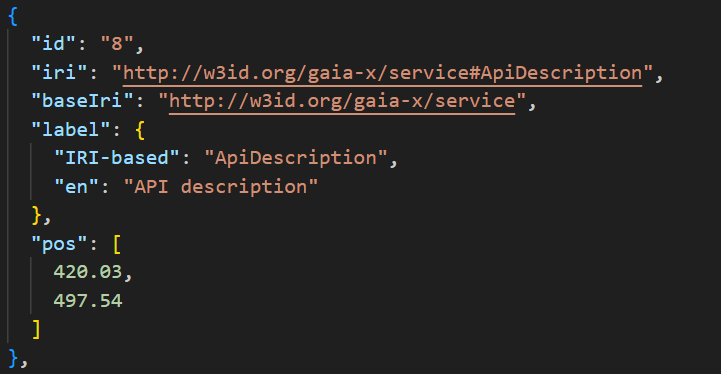
\includegraphics[width=0.7\linewidth]{chapter2/figures/position.png}
   \end{center}
   \caption[Objeto Json del archivo de posiciones]
   {\footnotesize Objeto Json del archivo de posiciones}
   \label{fig:mufigure13}
\end{figure}

\subsection{Exportación a archivos Jsonld}

El proceso de Exportación es muy similar, ya que leerá toda la información actual de cada burbuja en la escena y la guardará en un archivo json. Nuestro Parser tomará cada elemento y creará la clase Gaia-X correspondiente en un archivo jsonld. La lógica sigue siendo la misma, crear todas las clases y una vez que hayamos terminado, crear todas las conexiones.

Esta herramienta de Importación/Exportación es crucial para el proyecto. Sin ella, no tendríamos la interoperabilidad necesaria. Pero para ello, debemos estar seguros de que no estamos perdiendo información en ningún paso o dirección del proceso. Esto significa que tenemos que comprobar todas las listas con frecuencia y buscar anomalías y datos irregulares.

Una vez que terminemos las principales tareas de visualización, podremos enfocarnos en tareas de edición y creación por lo que las ontologías sufrirán modificaciones dentro de nuestra aplicación y si esta herramienta funciona correctamente, deberíamos ver los resultados en los archivos exportados.

\subsection{Contenedores de Ontologías}

La idea de esta característica es tener un contenedor para cada ontología de manera que podamos diferenciarlas fácilmente. Cada uno de ellos también debe ser interactivo para que pueda agarrarlos y moverlos en la escena, y al hacerlo, todas las clases contenidas se moverán de la misma manera. Esto creará una nueva capa de interacción en nuestra simulación, permitiéndonos interactuar tanto con burbujas como con ontologías completas. A partir de aquí, podemos añadir nuevas características que también se aplican a todas las clases de una ontología.

Este diagrama de clases nos muestra cómo están conectados los scripts en el código. OntologyManager se encarga de instanciar los prefabs y rellenar las listas correspondientes de cada uno de los subgestores.

Cada vez que creamos una nueva burbuja debemos comprobar si la ontología a la que pertenece ya existe y crearla en caso contrario. Cada nueva clase está contenida en un objeto con el nombre de la ontología y este a su vez está vinculado a de mayor jerarquía. Este último tiene 2 componentes de script: Ontologies.cs y ContainersManager.cs. Cada vez que tenemos que instanciar una nueva ontología, tenemos que añadirla a la lista de ontologías en Ontologies.cs y luego instanciar el contenedor y añadirlo a la lista ontologyContainers en el ContainersManager.cs

\begin{figure}[ht]
   \begin{center}
      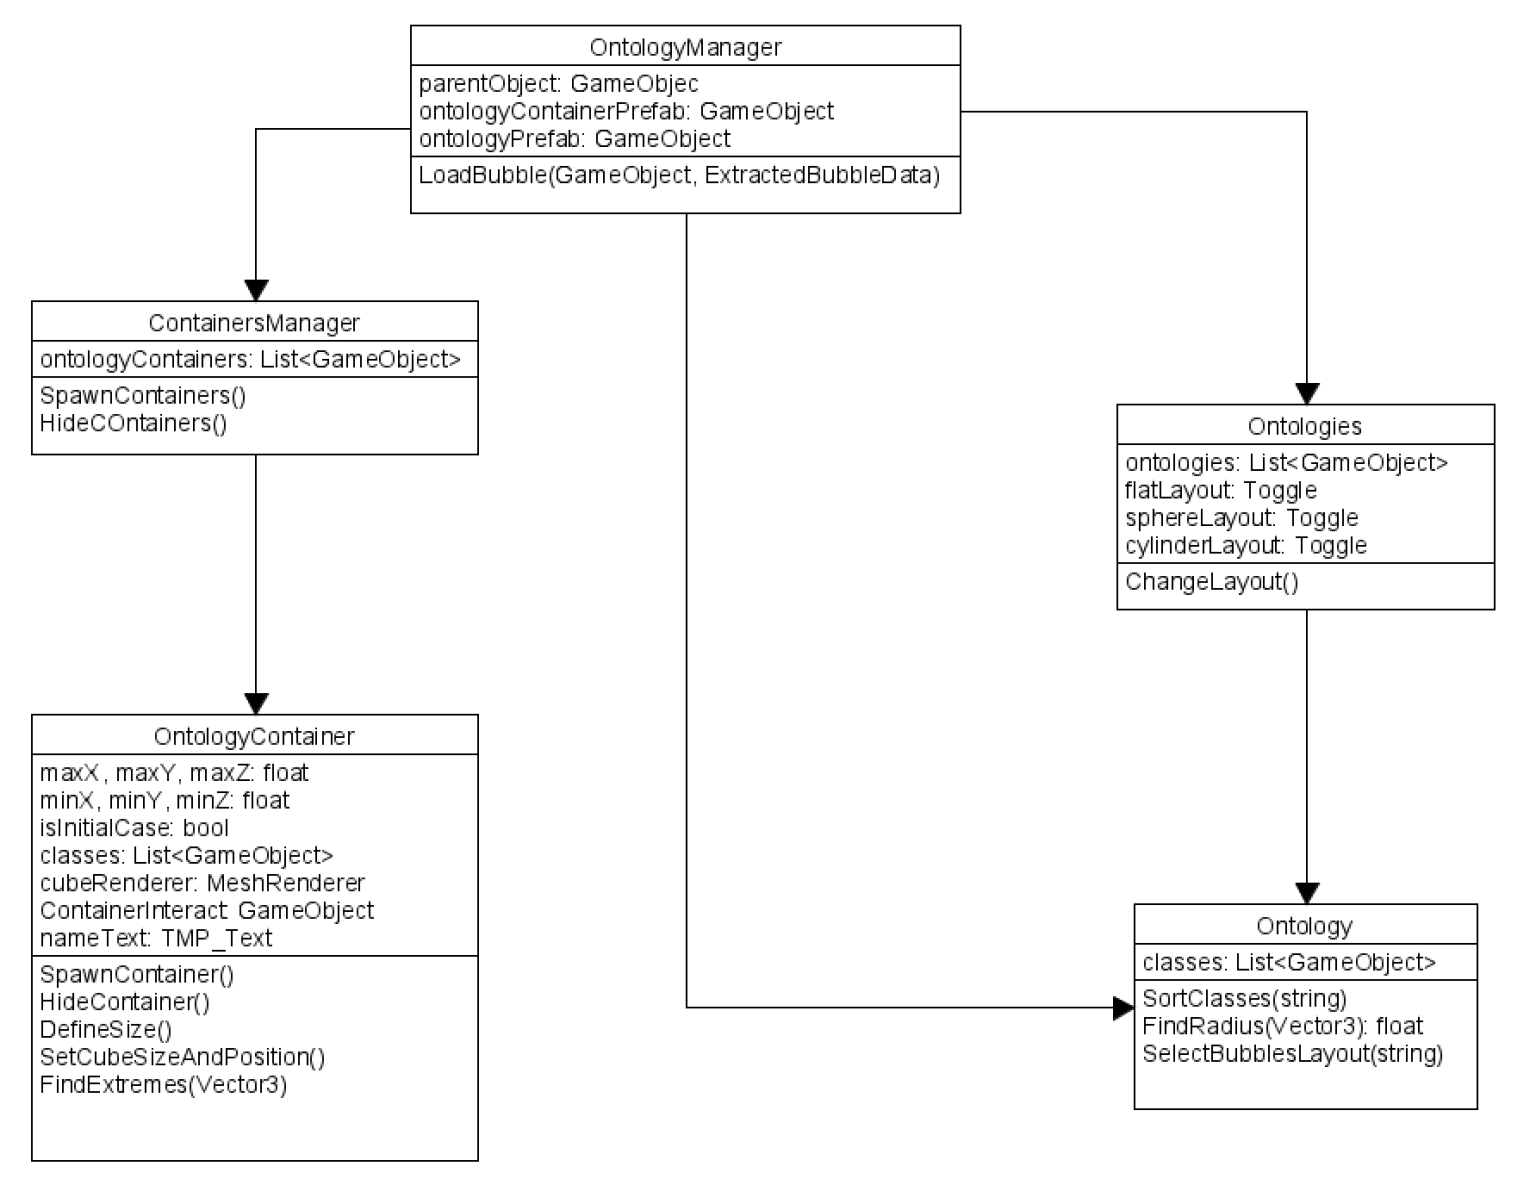
\includegraphics[width=1\linewidth]{chapter2/figures/containers.png}
   \end{center}
   \caption[Diagrama de clases para los contenedores]
   {\footnotesize Diagrama de clases para los contenedores}
   \label{fig:mufigure16}
\end{figure}

ContainersManager.cs tiene el control de la característica, por lo que es el componente que necesitamos para los métodos de callback.

OntologyContainer.cs tiene el control del propio contenedor, de forma que cada vez que decidamos generarlos, recalculará el tamaño de todas las burbujas. Los métodos son bastante sencillos de entender, pero el proceso es el siguiente: primero echamos un vistazo a todas las clases dentro de una ontología y encontramos los extremos de la misma (min y max de los 3 ejes). Con eso podemos saber el tamaño del propio contenedor y escalar el prefabricado para que se ajuste a la ontología. Ver código 2.3 del apéndice.

Cada contenedor también tiene un script VRInteractable para que podamos moverlo con el raycast de nuestro controlador. Lo bueno de esto es que cada clase contenida en él también se moverá en el mismo vector de desplazamiento y magnitud, por lo que todo se comportará como un bloque. Con esto conseguimos la capa de interacción mencionada anteriormente.

\begin{figure}[ht]
   \begin{center}
      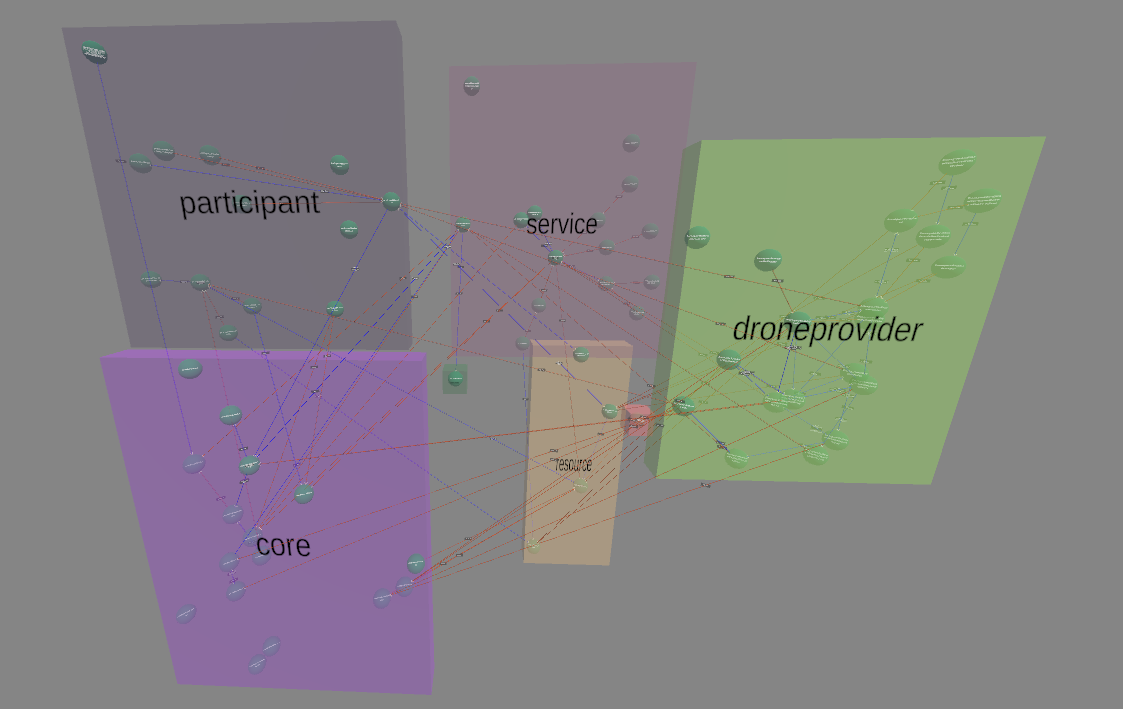
\includegraphics[width=0.8\linewidth]{chapter2/figures/ontologies&containers.png}
   \end{center}
   \caption[Ontologías y sus contenedores]
   {\footnotesize Ontologías y sus contenedores}
   \label{fig:mufigure17}
\end{figure}

\subsection{Modos de distribución de ontologías}

Esta característica pretende complementar el proceso de importación, ya que estamos asignando un valor de tercera dimensión al vector de posición para instanciar la burbuja, pero todas tienen el mismo, por lo que estamos perdiendo el efecto 3D del que estábamos tan orgullosos. Para superarlo, hablamos de utilizar formas geométricas básicas para describir cada ontología.
Calcularíamos la dimensión de la forma deseada y luego proyectaríamos cada clase según sus valores x e y. Ver código 2.4 del apéndice.

\begin{figure}[ht]
   \begin{center}
      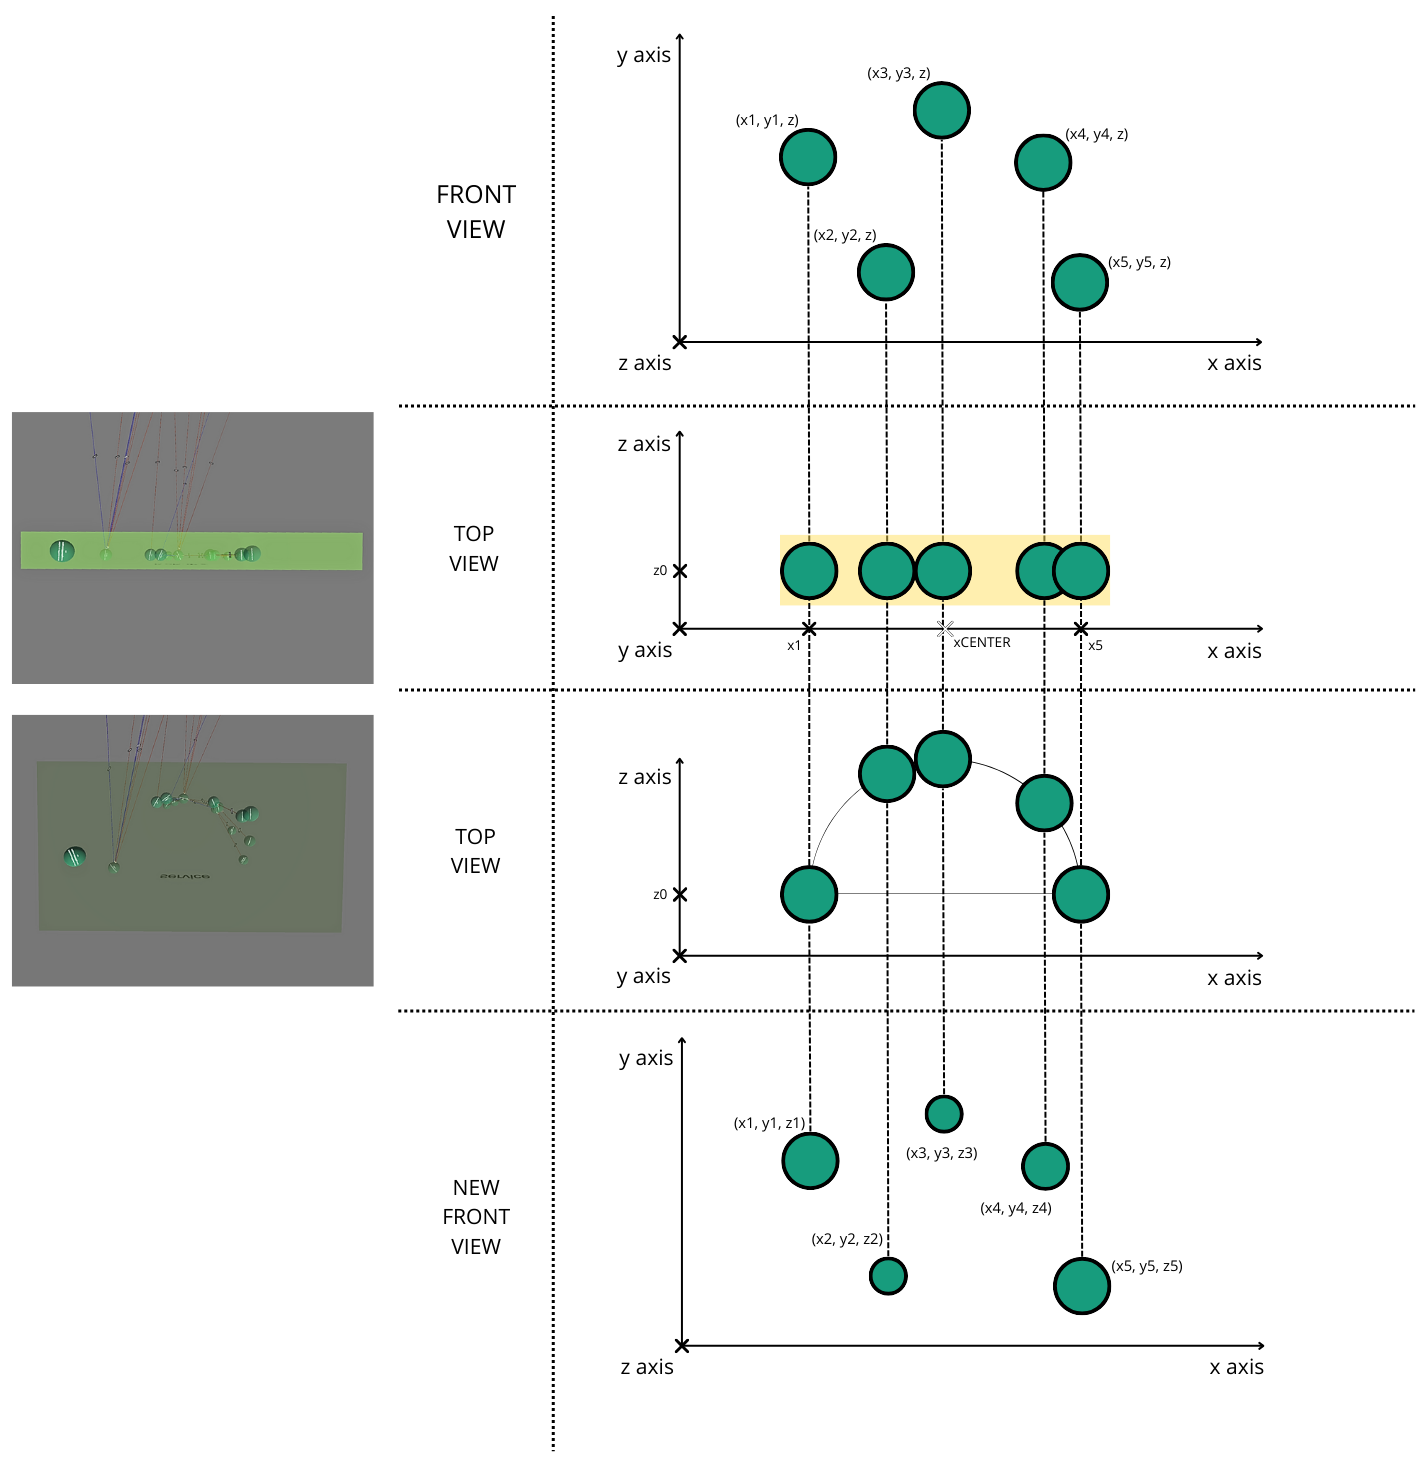
\includegraphics[width=0.8\linewidth]{chapter2/figures/clusters shape.png}
   \end{center}
   \caption[Cálculo de proyección para los modos de distribución]
   {\footnotesize Cálculo de proyección para los modos de distribución}
   \label{fig:mufigure17}
\end{figure}

En el caso de la Figura 2.14, tomamos la ontología y sus clases, calculamos la distancia x entre las burbujas más extremas, la utilizamos para crear un radio de cilindro y, a continuación, colocamos cada burbuja en el valor z de este cilindro según las otras dos coordenadas a modo de proyección.

Esta misma lógica se puede aplicar con cualquier forma deseada. También implementé una esférica pero no alcancé a hacerla funcionar correctamente antes del final de la pasantía. Si además añadiéramos rotaciones a las interacciones de los contenedores, podríamos buscar una forma ontológica concreta para colocarlos todos de la forma deseada y crear un layout mucho más agradable al usuario.

También podemos mencionar que, aunque estas distribuciones son puramente geométricas, también podríamos intentar dar con un parámetro que queramos optimizar y buscar un modelo de IA adecuado para ello. Por ejemplo, podría ser muy útil reducir la longitud total de las conexiones en la escena, de modo que no tengamos tantas líneas en la escena interfiriendo con los efectos visuales.


\clearemptydoublepage
\backmatter
\chapter*{Conclusiones}
\addcontentsline{toc}{chapter}{Conclusiones}
\chaptermark{Conclusiones}

El objetivo principal de estas prácticas era mejorar la herramienta 3D para visualizar ontología, con el fin de tener una alternativa a los softwares 2D tradicionales y evitar algunas limitaciones que normalmente tienen.
La primera fase estuvo orientada a filtrar las clases de la escena y desarrollar características para encontrar una clase lo más rápido posible. En noviembre, realizamos un estudio con distintos participantes del instituto
para recabar más información y comprobar el progreso actual de nuestro proyecto, y muchos de ellos afirmaron que la herramienta de búsqueda era increíblemente útil, y que el software de gestión ontológica no siempre dispone de una.

En el desarrollo de RV, cada herramienta tiene que probarse y analizarse desde diferentes perspectivas, ya que la mayor parte del tiempo nos ocupamos de la experiencia del usuario. Tenemos que implementar las cosas de forma que sean intuitivas para el usuario
y eso es algo que olvidamos más a menudo que nunca. Teníamos un miembro del equipo que se centraba exclusivamente en los prefabricados de interfaz de usuario, y teníamos que mantener actualizaciones constantes en nuestras ramas de trabajo con las versiones más recientes de los elementos de menú o interfaz de la escena.

También tuvimos que prestar mucha atención a la optimización para que la escena se ejecutara con la mayor fluidez posible y no rompiera la sensación de inmersión del usuario. Las simulaciones de RV dependen más del nivel de interacción entre el usuario y la escena que del realismo,
como mucha gente puede creer, así que todo tiene que funcionar de una manera muy específica para satisfacer al usuario. Se realizan pruebas con frecuencia para intentar encontrar fallos y posibles agujeros en el código.

Trabajar en equipo es todo un reto y exige desarrollar una gran capacidad de comunicación. Ser capaz de expresar lo que hay que hacer o sugerir nuevas ideas depende en gran medida de la forma en que exponemos lo que pensamos.

La documentación es una parte crucial de cualquier proyecto, ya que ayuda a los nuevos miembros del equipo y mantiene un control de versiones limpio. Dedicar tiempo a crear diagramas de clases, hacer capturas de pantalla y aclarar las conexiones de los inspectores entre los objetos del juego es la clave para
progreso claro. Una semana después de incorporar cada característica a la versión principal de la escena, se dedicó a documentar el trabajo realizado para esa cuestión.

\section{Trabajo Futuro}

El proyecto está lejos de estar terminado. Ahora que podemos importar y exportar información de los estándares de Gaia-X, podríamos pensar en añadir herramientas de edición a la escena.
Crear y borrar burbujas sería el primer paso, pero luego también tendríamos que añadir conexiones. Las clases deberían poder trasladarse de una ontología a otra, o incluso podrían crearse otras nuevas.

Como esta simulación forma parte del contexto del proyecto Gaia-X, también podríamos llevar a cabo más pruebas y recoger ideas de en qué sería importante centrarse a continuación. Algunas personas han sugerido añadir una función multijugador, de modo que podamos utilizar la simulación tanto
como una aplicación de coworking o como un tour de presentación. Esto significa que una persona interactúa con las ontologías y el resto observa lo que ocurre.

Se podría añadir otro intérprete para importar ontologías desde un formato de archivo diferente, como turtle. La idea es casi la misma que la que ya está implementada pero podría añadir mucha versatilidad al proyecto.

Como podemos ver, hay muchas cosas que se pueden hacer para seguir mejorando la simulación. La RV es una herramienta muy útil, pero aún no conocemos todo su potencial. Tenemos que seguir investigando, desarrollando y probando para encontrar nuevas formas de explorar la información.


% Chapitre pour la bibliographie
\clearemptydoublepage
\phantomsection % To have a correct link in the table of contents
\addcontentsline{toc}{chapter}{Bibliografía}

% nocite: Pour citer la totalit\'{e} des r\'{e}f\'{e}rences contenues dans le fichier biblio
% nocite: In order to cite all the references included biblio
\nocite{*}
\printbibliography

\end{document}
